% https://github.com/dcroote/stanford-thesis-example
% Friday Dec. 3rd noon

% Stanford University PhD thesis style -- modifications to the report style
% This is unofficial so you should always double check against the
% Registrar's office rules
% See http://library.stanford.edu/research/bibliography-management/latex-and-bibtex
% 
% Example of use below
% See the suthesis-2e.sty file for documentation
%
\documentclass[12pt]{report}
\usepackage{suthesis-2e}  % (modified) Stanford thesis style file

% useful packages
\usepackage{graphicx}  % figures
\usepackage{gensymb}  % \degree
\usepackage{siunitx}  % SI units
\usepackage{tabularx}  % nice single page tables
\usepackage{longtable}  % tables spanning multiple pages
\usepackage{hyperref}  % URLs
\usepackage[autostyle, english = american]{csquotes}  % quote orientation
\usepackage{epigraph}
\usepackage[ruled]{algorithm2e}
\usepackage{amsmath}
\usepackage{amssymb}
\usepackage[dvipsnames]{xcolor}
\definecolor{red}{HTML}{DB4437}
\definecolor{blue}{HTML}{4285F4}
\definecolor{yellow}{HTML}{F4B400}
\definecolor{green}{HTML}{0F9D58}
\renewcommand{\epigraphsize}{\normalsize}
\setlength{\epigraphwidth}{0.9\textwidth}
\MakeOuterQuote{"}

% use png first, otherwise pdf
% (useful for faster compile times, for final submission switch order)
\DeclareGraphicsExtensions{.png,.pdf}

\begin{document}
\title{Machine Learning Based Wavefront Sensing For The Rubin Observatory}
\author{David Thomas}
\dept{Computational and Mathematical Engineering}
\principaladviser{Professor Steven Kahn}
\firstreader{Professor Patricia Burchat}
\secondreader{Professor Stephen Boyd}

% no signature or copyright pages in online submission
% (they are added by the library)

% including chapters, no .tex extension necessary
\beforepreface
\afterpreface
\prefacesection{Abstract}
We present a new framework for wavefront sensing for wide-field telescopes. The framework divides the problem into two subproblems that are highly amenable to machine learning and optimization. The first involves making local wavefront estimates with a convolutional neural network. The second involves interpolating the optics wavefront from all the local estimates by minimizing a convex loss function. In this thesis, we develop simulated observations and images from the upcoming Rubin Observatory to refine and assess this framework. Much of this work is also summarized in \cite{2020SPIE11448E..4HT} and \cite{9523024}, although here we describe it in more detail. 

Our unique contributions are as follows. We isolated wavefront sensing problem and decomposed it into two sub-problems. We created benchmark datasets for both sub-problems. We demonstrated a convolutional neural network can predict local wavefront from donut images. We showed that the global wavefront can be interpolated with least squares from the local wavefront estimates. Finally, we developed a wavefront control simulation environment and used it to assess three canonical control strategies.

The algorithm has great practical properties - it is transparent, robust, low latency, and high bandwidth - and achieves stunning performance. In a realistic Rubin mini-survey, the algorithm reduces the total magnitude of the optics wavefront by 66\%, the optics PSF FWHM by 27\%, and increases the Strehl ratio by a factor of 6. The resulting sharper images have the potential to boost the scientific payload for astrophysics and cosmology.
\prefacesection{Acknowledgements}

The idea to pursue graduate school chrystalized when I was working as a quant for Teza Technologies, a small, academic high frequency trading firm. I witnessed first hand how machine learning and low latency technologies were completely up-ending securities trading. Broad shouldered Wall Street suites were being replaced by hackers and math nerds. As machine learning and automation became increasingly powerful tools for our firm, I began to question whether these tools could spur similar advances in physics and cosmology. 

In 2016, I started the ICME MS program and began working with Philip (Phil) Marshal on high dimensional cosmological inference. In the summer of 2017, Phil introduced me to my eventual advisor, Steven (Steve) Kahn, as someone who could potentially support me for a PhD. I remember our first meeting well. I presented my results. Steve sat there, completely silent. His stern expression gave no indications of his thoughts ... was he even paying attention? After I finished presenting, he asked extremely insightful questions that demonstrated he had been paying careful attention. Indeed, Steve is a great listener. I was also impressed by his creativity and interest in working on problems off the beaten path. Shortly after our first encounter we teamed up to work on star trails, and Steve officially became my PhD advisor. 

I would like to extend Steve my greatest thanks. The two major research efforts that comprise my PhD, star trail photometry and machine learning based wavefront sensing, were speculative and required many different attempts before we were ultimately able to crack them. Steve's patience and willingness to pursue bold problems made this possible. Great collaboration around AI. 

The two major research efforts that comprise my PhD, developing star trail photometry and machine learning based wavefront sensing algorithms, . The former is not a part of this PhD as I ran out of time to include it - we can save it for the journals.  

The other thing that stood out was Steve's creativity. . At the time, when I had struggled to sell other Physics professors on the implications of deep learning for physics - this is almost hard to believe today - . 


The 

It started at Teza Technologies, where I was a quant for three years. We had a lot of success developing machine learning algorithms and low latency technologies to trade futures.



Story.

First and foremost, I would like to thank Steve.

Mentors like Pat Burchat, Aaron Roodman, and Steven Boyd. 

Joshua Meyers. Federica Bianco. 

Bo Xin, Sandrine Thomas, Te Wei Tsai, Chuck Claver

Stanford University. Phd minors.

Family.

Wife.

(Facebook and Citadel. Both of these gave me ample experience, taught me about new industries, and provided me with valuable skills. )

Mentoring XY. 
% \include{ch_intro}
\part{Machine Learning Based Wavefront Sensing}
% Full title as you would like it to appear on the page
\chapter{A New Paradigm For Wide-Field Wavefront Sensing}
\label{chap:new_paradigm}
% Short title that appears in the header of pages within the chapter
\chaptermark{A New Paradigm}

\epigraph{What is the most important theme in computer science? [Class responds.] No. It is \textit{abstraction}.}{John Ousterhout in CS 140: Operating Systems, 2020}

\section{Challenges with Previous Approaches}

Keeping telescopes in focus is an art as old as the instruments themselves. Their widespread use spurred the development of theories of optics and aberrations. In 1678, the famed Dutch physicist Christian Huygens proposed that every point that interacts with light may be regarded as the source of a new spherical wave. In 1818, the French physicist Augustin-Jean Fresnel incorporated interference into this model. The resulting Huygens-Fresnel principle is still a widely taught model for wave propagation and provides the physical intution behind reflection, refraction, and diffraction. The paradigm also introduced the notion of the wavefront.

A wavefront is a two dimensional surface over which the phase of the wave is constant. We also overload this diction to refer to aberrations, or two dimensional spatial offsets from a reference wavefront. Figure \ref{fig:wavefront} shows example aberrations to planar and spherical reference wavefronts. 

\begin{figure}[hbt!]
\centering
\includegraphics[width=14cm, keepaspectratio]{figs/new_paradigm/wavefront.png}
\caption[Wavefront and Wavefront Aberrations]{Example aberated planar and spherical wavefronts. The horizontal red lines show the direction of propagation. The vertical red line shows the reference wavefront and the blue line shows an example aberrated wavefront. Source: \cite{wavefront_fig}. }
\label{fig:wavefront}
\end{figure}

Wavefronts are useful because the wavefront aberrations in different planes, and through time, largely characterize the image quality of an optic. In the case of ground based telescopes, there are three primary contributions to image quality: the atmosphere, the telescope, and the camera. The field of \textit{adaptive optics} is concerned with controlling deformable mirrors to the optical path to correct for aberrations induced by atmospheric turbulence on 10-100Hz frequencies. However, for wide field telescopes with fields of view on the order of a degree, a common corrections is not possible for the entire field of view. In this context we are primarily concerned with \textit{active optics} which strives to correct the aberrations due to the telescope. New methods of wavefront sensing for active optics is the focus of the first part of this thesis.

One way to characterize the optics of a telescope is through path length differences. For every position in the image plane, we can measure the path differences to points in the entrance pupil. An alternative way to mathematically express this is through an aberrated wavefront defined at the entrance pupil for each position in the image plane. Then the imaging properties can be computed with Fourier Optics. We refer readers who would like to understand this relation further to Goodman's classic Fourier Optics text \cite{goodman2005introduction}. 

There are two thematic approaches to wide field wavefront sensing: zonal and modal. In the zonal approach, the entrance pupil is partitioned into an array of subaperatures. In each of these zones, the wavefront is characterized by its optical path length, local gradient, or local curvature. The wavefront measurement improves with more partitions. The Shack-Hartmann sensor and shearing interferometer are the two most common zonal approaches.

The modal approach treats the wavefront aberration, at a given point in the image plane, as a sum of low order polynomials defined over the entrance pupil. This wavefront measurement improves with higher order polynomial measurements. Modal approaches typically rely on strategically defocused wavefront sensors. The Rubin Observatory focal plane was designed with a modal approach in mind as it does not require lenselets or tweaks to the beam. As described in chapter \ref{chap:aos}, the Rubin focal plane contains four corner wavefront sensors specifically for this purpose.

There are two previously described approaches to wavefront sensing that are relevant for Rubin. The first, by Roodman et. al. \cite{2014roodman}, is the algorithm used for the Dark Energy Camera on the Blanco Telescope \cite{darkenergycamera}. It is based on the Fraunhofer diffraction integral:

\begin{equation}\label{eqn:fraunhofer}
I(x,y) \propto |\mathcal{F}\{P(\rho, \theta \exp(2\pi i W(\rho, \theta) / \lambda))\}|^2
\end{equation}

\noindent where $I$ is intensity; $\mathcal{F}$ is the two-dimensional Fourier transform; $P$ is the pupil function; $W$ is the wavefront; $\lambda$ is the wavelength; and $x,y$ and $\rho, \theta$ parameterize the image and pupil planes respectively. The wavefront is modeled as a sum of orthonormal Zernike polynomials:

\begin{equation}\label{eqn:zernike_decomp}
W(\rho, \theta) = \sum_i a_i Z_i(\rho, \theta)
\end{equation}

\noindent Starting from a set of telescope control parameters, the wavefront coefficients can be computed. Then the Fraunhofer diffraction integral can be used to generate a corresponding intensity image. The difference between the donut images and the images from the forward model,

\begin{equation}\label{eqn:loss}
\mathcal{L} = \sum_{\text{donut d}}||I_{\text{d,true}} - I_{\text{d,forward}}||_2^2
\end{equation}

\noindent can be used as a loss function. Then we can estimate the telescope parameters by using an optimizer to find the parameters that minimize this loss function. This works well when there are a few non-degenerate parameters and the problem remains approximately convex.

While this approach has been successfully applied to the Blanco Telescope, there are two impediments to applying it to the Rubin Observatory. The first is that Rubin has much higher dimensionality and complete degeneracy between some of the parameters of interest. The Blanco Telescope is a prime focus telescope with a single mirror; the Rubin Observatory is a modified Paul-Baker telescope with three mirrors. The Blanco active optics sytem controls 8 parameters; the Rubin active optics system strives to control 50 parameters. The Rubin control parameter optimization surface is highly nonconvex. In addition to these theoretical hurdles, the fast beam of the Rubin optics also necesitates much larger fourier transforms pushing the runtime of the algorithm beyond the 15 seconds we are targeting (see next chapter for more details). 

The second approach is based on the transport of intensity equation (TIE):

\begin{equation}\label{eqn:tie}
\frac{\partial I}{\partial z} = -(\nabla I \cdot \nabla W + I \nabla^2 W)
\end{equation}

\noindent where $z$ is the optical axis. It builds on the curvature wavefront sensing technique developed by Francois, Claude, and Nicolas Roddier \cite{curvaturesensing}. Their key insight was that $\frac{\partial I}{\partial z}$ can be approximated by subtracting two donut images on different sides of focus. Then $W$ in the TIE equation can be solved for in Fourier space or with a Zernike polynomial series expansion. The large central obscuration, fast $f$-number, off-axis distortion and vignetting, and different field positions of intra and extra-focal donuts are four challenges to using curvature sensing for Rubin. Xin et. al. \cite{2015Xin} proposed solutions and extended curvature sensing to estimate the Rubin optics wavefront at four field positions. Below we give a high-level summary of the operations this algorithm performs, on a single wavefront sensor, to estimate the wavefront at the center of the corresponding wavefront sensor:

\begin{enumerate}
\item Crop $N$ pairs of intra-focal and extra-focal donuts \\$\{(D_{\text{intra},1},\ D_{\text{extra},1}), \dots, (D_{\text{intra},N},\ D_{\text{extra},N})\}$.
\item Make initial wavefront estimates $W_0 = 0,\ W_1 = \text{guess}$.
\item Set $i = 1$.
\item While $||W_i - W_{i-1}||_2^2 < \text{tolerance}$ repeat,
\begin{enumerate}
\item Apply nonlinear transformation $f$ which migrates donut image from its field position to the center of the wavefront sensor, based on current wavefront estimate $W_i$. We have $\{(D_{\text{intra},1}^\prime,\ D_{\text{extra},1}^\prime), \dots, (D_{\text{intra},N}^\prime,\ D_{\text{extra},N}^\prime)\}$ where $D_{*,k}^\prime = f(D_{*,k}, W_i)$.
\item Apply correct $g$ for intensity and vignetting differences between the pairs of donuts. We have $\{(D_{\text{intra},1}^{\prime\prime},\ D_{\text{extra},1}^{\prime\prime}), \dots, (D_{\text{intra},N}^{\prime\prime},\ D_{\text{extra},N}^{\prime\prime})\}$ where $D_{*,k}^{\prime\prime} = g(D_{*,k}^\prime, W_i)$.
\item Set $(\partial_z I)_k \propto D_{\text{intra},k}^{\prime\prime} - D_{\text{extra},k}^{\prime\prime}$.
\item Solve TIE for $W_{i+1}$ with $(\partial_z I)_k$ by series expansion.
\item Set $i = i + 1$.
\end{enumerate}
\item Return $W_i$ as wavefront for the center of the wavefront sensor.
\end{enumerate}

\noindent Afer this process the algorithm uses the wavefront estimates at the center of the four corner wavefront sensors to constrain 50 telescope control parameters (these parameters are described in the next chapter). 

This approach has been developed by a dedicated team over the last decade. Parts of the algorithm, such as step 4 (d) are mature and have been validated on real data \cite{cwfs_comparison}. However, despite significant effort, the code for the full algorithm on Rubin remains incomplete. Thus it is difficult to benchmark or compare to alternatives.

The primary challenge on theoretical grounds is the convergence. There are no convergence gaurentees. The wavefront estimate may not improve between the iterations in step 4. Some tests suggest that the algorithm typically converges for small perturbations to the nominal optics configuration. However, for large perturbation the transformations $f$ and $g$ will have more error. A different strategy might be required.

The algorithm is also fairly computationally expensive. It takes approximately 15 seconds to perform 10 iterations of step 4 on 10 pairs of donuts. However, a typical wavefront sensor image contains close to a thousand donut images. A lot of potentially useful donut information is ignored.

There are also a few challenges on practical grounds. The functions $f$ and $g$ used in step 4 depend on the wavefront estimate and are fairly complicated. This makes the algorithm challenging to interpret and debug. Also, since $f$ and $g$ depend on the wavefront estimate, it is difficult to characterize the error in the full algorithm, because each step depends on the preceeding steps. 

After spending a year supporting efforts to implement this algorithm, I realized the prudence in developing an alternative approach. I sought to develop an algorithm that was simple, transparent, robust, low-latency, and high-throughput. The next two sections develop two key paradigms behind the algorithm.

\section{The Double Zernike Polynomials}

The Zernike polynomials are a sequence of polynomials $\{Z_i\}$ that are widely used to characterize wavefronts in optics \cite{zernike}. They are defined over a unit disk, or annulus, and normalized such that

\begin{equation}\label{eqn:zernike_norm}
\int_{R_{\text{inner}}}^{R_{\text{outer}}} \int_0^{2\pi} Z_i(\rho,\theta)Z_j(\rho,\theta)d\rho d\theta = \delta_{ij}
\end{equation}

\noindent Figure \ref{fig:zernike} shows the first 21 Zernike polynomials. For characterizing a wavefront in the pupil plane we follow the convention of using $Z_4-Z_{21}$ by Xin et. al. \cite{2015Xin}. The first three polynomials are ignored because while they effect the position of the image, they do not impact the image quality. The polynomials beyond 21 are ignored because they are only weakly excited by typical Rubin perturbations.

\begin{figure}[hbt!]
\centering
\includegraphics[width=14cm, keepaspectratio]{figs/new_paradigm/zernikes.png}
\caption[Zernike polynomials]{The Zernike polynomials $Z_1$ throught $Z_24$ with the Noll index scheme. The obscuration of the annular domain is consistent with the obscuration in the Rubin optics.}
\label{fig:zernike}
\end{figure}

For small telescopes, this basis can be used to characterize the wavefront in the entrance pupil. For wide-field telescopes like the Rubin Observatory, the wavefront changes non-trivially across the field of view. Thus the wavefront is a four dimensional function of both the entrance pupil and focal plane. One way to model this would be to have another polynomial basis $\{P_i\}$ for the focal plane $x,y$. Then we could write the full wavefront as $W(x,y,\rho, \theta) = \sum_i \sum_j \beta_{ij} P_i(x,y) Z_j(\rho, \theta)$. The coefficients $\beta$ are indexed by the image plane index $i$ and pupil plane index $j$. The double Zernike polynomials are the $P_i(x,y) Z_j(\rho, \theta)$ where the field polynomials are circular Zernike polynomials $P_i = Z_i$ \cite{doublezernike}. Thus $\beta_{ij}$ is the mode of circular polynomial $Z_i$ in the focal plane, and annular polynomial $Z_j$ in the image plane.

In practice we also truncate the focal plane index. This leaves us with a finite set of coefficients to represent the full wavefront across the pupil and focal planes. We found that for the Rubin Observatory, most of the aberration power is concentrated in the first three focal plane polynomials. We simulated 500 perturbed telescope states and numerically calculated the double Zernike coefficients out to index 36. Then we studied the fraction of the aberrated wavefront contained in the first $k$ focal plane Zernikes. We found that the first three polynomials capture 90\% of the wavefront. These first three polynomials are a constant offset, a tip-plane, and a tilt-plane - collectively they define a plane. We suspect a similar pattern holds for other wide field telescopes. It suggests that the 54 double Zernike coefficients $\beta_{ij}$where $1 \leq i \leq 3$ and $4 \leq j \leq 24$ offer a good characterization of the wavefront.

\begin{figure}[hbt!]
\centering
\includegraphics[width=14cm, keepaspectratio]{figs/new_paradigm/truncated.png}
\caption[Aberration Power in Focal Plane Zernikes]{The fraction of the aberration that is present in the first $k$ focal plane Zernike polynomials, where $k$ is the truncation index on the x-axis.}
\label{fig:truncated}
\end{figure}

This separation of the wavefront into pupil and focal plane components is key to this work. Our key insight was as follows. At any point in the image plane, we can use the image to constrain the pupil wavefront at that position - we deem this the \textit{local} wavefront. Then we can interpolate the focal, or \textit{global}, wavefront from all the local estimates. In section \ref{sec:decomposing}, we describe techniques that are very well suited for each of these subproblems. Before then, we summarize recent progress in neural network based phase estimation.

\section{Neural Network Based Phase Estimation}
The potential for neural networks to learn the non-linear mapping between intensity patterns and aberrations in the pupil plane was first recognized in 1990 \cite{1990NatureMLAO}. Shortly afterwards, this potential was realized as neural networks were deployed to detect turbulence induced distortion on the Multiple Mirror Telescope \cite{1991NatureMLAO} and to detect aberrations in the primary mirror of the Hubble Space Telescope \cite{1993HubbleMLAO}. Others expanded this concept to predict more wavefront components \cite{1992SPIE.1706..113J}, incorporate temporal history \cite{1996ESOC...54...95L,1997ApOpt..36..675M}, compare reconstruction methods \cite{2006OExpr..14.6456G}, and better characterize atmospheric turbulence \cite{2008ISTSP...2..624W}. 

In the past decade, convolutional neural networks (CNNs) \cite{726791} have re-emerged and spurred dramatic advances in computer vision \cite{10.5555/2999134.2999257, 10.5555/2999792.2999897, 10.1007/s11263-015-0816-y,7780459}. This has created new possibilities for wavefront sensing in astronomy. In \cite{2018OptL...43.1235P}, the authors created a CNN that could estimate the wavefront from a single PSF image. They used these estimates as initial starting points in a gradient-based optimization and showed this was superior to using random samples. \cite{2019OExpr..27..240N} showed wavefront sensing performance could be improved by introducing a preconditioner to broaden the PSF and create more intensity structure for the neural network to exploit. This brings up interesting new design possibilities for wavefront sensors. While conventional Lyot-based low order wavefront sensing methods have a limited dynamic range due to their linear recovery, \cite{2020OExpr..2826267A} showed that a CNN can extend the aberration range over which the wavefront can be estimated by an order of magnitude.

Previous work on machine learning based wavefront sensing focuses on sensing the full wavefront aberration. Here we focus on sensing the optics wavefront, across the field of view, in the midst of the dominant atmospheric contribution. This problem presents new challenges, such as how to best aggregate intensity information from throughout the field of view to suppress the spatially correlated error due to the turbulence contribution. Our approach is comprised of only two steps, is easy to characterize, and can process each donut image in 6 \textit{milliseconds}.

\section{Wavefront Estimation Framework}
\label{sec:decomposing}

The optics wavefront $W_{\text{opt}}$ is a function of two separate planes: the pupil plane parameterized by $(u,v)$ and the focal plane parameterized by $(x,y)$. We use the double Zernike polynomial basis \cite{doublezernike} to represent the optics wavefront, 
\begin{equation}W_{\text{opt}}(u,v,x,y) = \sum_{i=1}^k\sum_{j=1}^m\beta_{ij}Z_i(u,v)Z_j(x,y)\end{equation}
\noindent where $\beta_{ij}$ are the coefficients, $Z_i$ are annular Zernike polynomials over the pupil, and $Z_j$ are circular Zernike polynomials over the focal plane. The goal of wavefront sensing is to estimate these coefficients $\beta_{ij}$ from the $n$ donut images $D_i$ positioned across the wavefront sensors (see Figure \ref{fig:focalplane}). Let the position of donut $i$ be $x_i,y_i$ and the defocus offset of the corresponding sensor be $z_i$. The wavefront sensing problem is to find $f$ such that
\begin{equation}\beta = f((D_1,x_1, y_1, z_1), \dots, (D_n, x_n, y_n, z_n))\end{equation}

We break this into two subproblems.

\begin{enumerate}
	\item Estimate the local wavefront with a CNN at each donut position.
	\item Interpolate the global wavefront from the local wavefront estimates across the focal plane.
\end{enumerate}

\noindent These steps are outlined in Figure \ref{fig:twostep}. 

\begin{figure}[hbt!]
\centering
\includegraphics[width=14cm, keepaspectratio]{figs/new_paradigm/twostep.png}
\caption[Two Step Approach To Wavefront Sensing]{In the first step, a convolutional neural network (CNN) processes each donut crop on the four wavefront sensors. In the second step, from each local wavefront coefficient we interpolate three global wavefront coefficients with least squares optimization (LS).}
\label{fig:twostep}
\end{figure}

\subsection{Estimating Local Wavefronts}
In the first subproblem, we estimate the total local wavefront $w_{\text{tot}}(u,v)$ from donut $D_i$ at position $x_i, y_i, z_i$. The intensity in the donut image is related to the total local wavefront by the Fraunhofer diffraction integral (equation \ref{eqn:fraunhofer}). We represent the local wavefront in a basis of annular Zernike polynomials over the pupil, such that the total local wavefront for donut $i$ at position $x_i, y_i$ is
\begin{equation}
w_{\text{tot}}(u,v) = \sum_j \alpha_{ij}Z_j(u,v)
\end{equation}
Convolutional neural networks (CNNs) are particularly well suited for processing images and learning nonlinear mappings. We develop a CNN $\varphi$ to solve the inverse problem of estimating $\alpha_{ij}$ for $j = 1\ \dots m$ from $(D_i,x_i,y_i,z_i)$ . In chapter \ref{chap:cnn} we describe the implementation of this model in detail. 

\subsection{Interpolating the Optics Wavefront}

In the second subproblem, we aggregate the local estimates from the first subproblem to constrain $\beta$. The total local wavefront at position $x_i,y_i$ is related to the optics wavefront via
\begin{equation}w_{\text{tot}}(u,v) = W_{\text{opt}}(u,v|x_i,y_i) + \epsilon(u,v|x_i,y_i)\end{equation}
where $\epsilon$ represents the atmospheric turbulence contribution to the wavefront. Let $\mathcal{Z}$ be defined such that $\mathcal{Z}_{ij} = Z_j(x_i,y_i)$. Then for $i = 1,\dots,m$ we have
\begin{equation}
\alpha e_i = \mathcal{Z} \beta e_i + \epsilon
\end{equation}
where $e_i$ is the $i$th unit vector. Then combining the $\alpha$ from the previous subproblem, and computing the corresponding $\mathcal{Z}$, allows us to solve for $\beta$,
\begin{equation}
\beta = \text{argmin}_{\beta}\left \{\sum_{i=1}^m \ell(\alpha e_i, \mathcal{Z} \beta e_i)\right\}
\end{equation}
where $\ell$ is a convex loss function. Algorithm \ref{alg:main} shows the psuedocode. 

\begin{algorithm}
    % \SetKwInOut{Input}{Input}
    % \SetKwInOut{Output}{Output}
    % \underline{function Estimate Optics Wavefront}\\
    % \Input{combined wavefront sensor image $I \in \mathbb{R}^{N\times N}$}
    % \Output{optics wavefront $\beta \in \mathbb{R}^{k \times m}$}
    \text{given image} $I \in \mathbb{R}^{N \times N}$\\
    \text{initialize local wavefront estimate} $\alpha \in \mathbb{R}^{n \times m}$\\
    \text{initialize global Zernike basis} $\mathcal{Z} \in \mathbb{R}^{n \times k}$\\
    \For{\text{donut} $i$ \text{ in } 1\dots n}
    {
        $D_i = \text{Crop}(I, x_i, y_i)$\\
        $\alpha[i,:] = \varphi(D_i, x_i, y_i, z_i)$\\
        \For{\text{Sernike} $j$ \text{ in } 1\dots k}
        {
        	$\mathcal{Z}[i,j] = Z_j(x_i, y_i)$
        }
    }
    \text{initialize optics wavefront} $\beta \in \mathbb{R}^{k \times m}$\\
    \For{\text{local Zernike } $i$ \text{ in } $1 \dots m$}
    {
      $\beta[:,i] = \text{argmin}_{\beta[:,i]}\ \{\ell(\alpha[:,i], \mathcal{Z}\beta[:,i])\}$\\
    }
    \text{return } $\beta$\\
    \caption{estimates the optics wavefront from donut images.}
    \label{alg:main}
\end{algorithm}

The dominant source of error is the atmospheric turbulence contribution to the wavefront. This error is correlated on scales of arcminutes. By processing donuts with reasonable separation and between different wavefront sensors we are able to suppress this error by roughly a factor of $1 / \sqrt{n}$ where $n$ is the number of donuts used.

There are two parameters of our algorithm that must be set based on the telescope: the number of Zernike coefficients to use for the pupil $m$, and the number of Zernike coefficients to use for the focal plane $k$. For the Rubin Observatory we use Zernikes $Z_4$ through $Z_{21}$ for the pupil plane. The first three coefficients do not impact image quality, so we exclude them. We truncate the basis at $Z_{21}$, a convention set by \cite{2015Xin}, as the higher order terms have very small coefficients in practice. We use $Z_1$ through $Z_3$ for the focal plane. Our simulations show that 90\% of the optics wavefront is contained in this truncated basis.

There are two benefits to dividing the wavefront estimation problem into these two subproblems that are worth highlighting. The first is the useful intermediate data products. The local wavefront coefficients $\alpha$, which are estimated in the first subproblem, are physically meaningful. Telescope operators can track them during operations and gain further insight into the system. This adds an additional layer of transparency and robustness.

The second benefit is that it makes deep learning approaches feasible. Deep neural networks must be trained on large datasets to avoid overfitting. The input to the original problem is four wavefront sensor images, or up to thousands of donut images. The raytracing necessary to simulate even a single input sample is computationally expensive. In our first subproblem however, the input is only a single donut image. This reduces the computation required to produce a training sample by three orders of magnitude and makes it possible to generate simulated datasets that are sufficient for training deep neural networks. In chapter \ref{chap:cnn}, we highlight the power of these models.


% Full title as you would like it to appear on the page
\chapter{The Rubin Observatory Active Optics System}
\label{chap:aos}
% Short title that appears in the header of pages within the chapter
\chaptermark{Rubin Active Optics}

\epigraph{Some people don't like change, but you need to embrace change if the alternative is disaster.}{Elon Musk}

\section{Rubin Telescope}
The Vera C. Rubin Observatory is a 8.4-m wide-field telescope designed to measure the structure and evolution of the universe. The roots of the observatory date back twenty years ago to a 2001 proposal for The Dark Matter Telescope \cite{2001ASPC..237..417T}. The original scientific motivation was to produce premier weak lensing catalogs. Since then, the facility has gone through two name changes (it was the Large Synoptic Survey Telescope for many years) and the purview has expanded to include cataloging the solar system, mapping the milky way, and exploring the transient and variable sky \cite{sciencebook}. Site construction began on Cerro Pach\'{o}n, Chile in 2015 and is expected to be completed in 2023 \cite{2020SPIE11445E..0IT, 2020SPIE11445E..1US}. 

Rubin will have a $319\ \text{meter}^2\text{degrees}^2$ \'{e}tendue, ten times larger than any previous or currently planned telescope. The large \'{e}tendue is achieved by a novel three mirror design with a very fast f/1.234 beam. The design is optimized to attain seeing limited image quality across the $9.6\ \text{deg}^2$ field of view and passband spanning $320-1050\ nm$. Figure \ref{fig:telescope} shows the light path through the optics. The incident light first strikes the annular primary mirror M1, which has an outer diameter of $8.4\ m$ and an effective filled aperture of $6.4\ m$. Next the light visits the $3.4\ m$ convex secondary mirror M2 and the $5.0\ m$ concave tertiary mirror M3. Then the light passes through three refractive camera lenses and onto the $64\ cm$ focal plane. 

The primary and tertiary mirrors, M1 and M3, share an inner and outer radius respectively. This was chosen so that they could be fabricated from a single monolithic blank using spin-cast borosilicated technology. We refer to this collective mirror as M1M3. 

\begin{figure}[hbt!]
\centering
\includegraphics[width=14cm, keepaspectratio]{figs/rubin_telescope_and_aos/telescope.png}
\caption[Rubin Optics]{The optic elements of the Rubin telescope. The light path through the optics is shown in orange.}
\label{fig:telescope}
\end{figure}

\section{Active Control}

There are two telescope properties that incentivize the creation of telescopes with large primary mirrors. First, the \'{e}tendue, or light collecting power of a telescope is proportional to the area of the primary mirror. Second, the diffraction limited seeing is inversely proportional to the diameter of the primary mirror. Historically these primary mirrors were thick in order to maintain their nominal surface figure. However, the maximum size possible by these manufacturing processes is 5-6 meters of diameter.

In the late 1980s active optics technology was developed to enable the construction of a generation of telescopes with 8 meter primary mirrors. The mirrors for telescopes with this technology are thin and malleable. For Rubin, the mirrors are made out of borosilicate, which also quickly equilibrates with the ambient temperature. Active optics works by actively adjusting degrees of freedom of the telescope, including the mirror surface, based on a feedback system. The main sources of deviation to correct for are mechanical stresses stemming from the dyamics, wind, and gravity and temperature gradients in the mirror surfaces.

Figure \ref{fig:m1m3act} shows the active components of the combined primary and tertiary mirrors M1M3. The position in the x,y, and z directions is controlled by six large actuator hardpoints that form a hexapod. The mirror surface is controlled by 156 pnuematic actuators. The distribution of the actuators and their axes is explained in detail in \cite{2016SPIE.9906E..0QN}, although these details are not critical for this thesis. Given that even the large hardpoint acutators are pneumatic it is apt to say that the mirror sits on air. 

\begin{figure}[hbt!]
\centering
\includegraphics[width=14cm, keepaspectratio]{figs/rubin_telescope_and_aos/M1M3actuators.png}
\caption[Rubin M1M3 Hexapod and Pneumatic Actuators]{View of the bottom face of the M1M3 mirror showing: (a) pneumatic figure control actuators and (b) hard point hexapod. Source: \cite{2016SPIE.9906E..0QN}.}
\label{fig:m1m3act}
\end{figure}

Figure \ref{fig:m2act} shows the active components of the aspherical secondary mirror M2. The position in the x,y, and z directions is controlled by six large tangential electromechanical actuators. The mirror surface is controlled by 72 axial electromechanical actuators. The details of the configuration, metrology, and testing are described further in \cite{2016SPIE.9906E..67N}. Again, these details are not strictly necessary for what follows.

\begin{figure}[hbt!]
\centering
\includegraphics[width=14cm, keepaspectratio]{figs/rubin_telescope_and_aos/M2actuators.png}
\caption[Rubin M2 Hexapod and Mechanical Actuators]{Top and bottom views of the secondary mirror M2 showing the mirror cell, mirror, axial actuators, and tangential hard points. Source: \cite{2016SPIE.9906E..67N}.}
\label{fig:m2act}
\end{figure}

While it is important to understand the underlying physical interfaces for controlling the telescope, we use a key abstraction to reduce the dimensionality of the problem. Instead of modeling the state of the mirror surfaces with hundreds of predicted actuator deviations, we use low order bending modes. These are the modes that are most excited by the aforementioned sources of perturbations. Not only does this allow us to reduce the dimensionality by an order of magnitude, it also better captures the deviations we care about. We use finite element simulations to determine which modes have the most power and how many modes are required to maintain Rubin image quality specifications. 

At the time this work was initiated, all the bending modes had not been confirmed. Thus we decided to parameterize deviations to the mirror surface with the first 20 annular Zernike polynomials. We do not belive this choice has significant impact on the analysis. Table \ref{tab:dof} shows the 50 degrees of freedom - 5 for each hexapod and 20 for each mirror surface. It is worth emphasizing that this telescope's predecessor, the Dark Energy Camera on the Blanco Telescope, only controls 8 degrees of freedom. 

\begin{table}[hbt!]
\caption[The 50 Telescope Degrees of Freedom]{\label{tab:dof}The 50 telescope optics control parameters. Notation: dx is a translation in the x-axis and rx is a rotation along the x-axis.} 
\begin{center}
\begin{tabular}{|l|l|}
\hline
\rule[-1ex]{0pt}{3.5ex} Camera hardpoints & dx, dy, dz, rx, ry \\
\hline
\rule[-1ex]{0pt}{3.5ex} M2 hardpoints & dx, dy, dz, rx, ry \\
\hline
\rule[-1ex]{0pt}{3.5ex} M1M3 figure & 20 surface bending modes \\
\hline
\rule[-1ex]{0pt}{3.5ex} M2 figure & 20 surface bending modes \\
\hline
\end{tabular}
\end{center}
\end{table} 

\section{Wavefront Sensors and Donut Images}

In the last section we discussed the degrees of freedom we are trying to predict and control. In this section we describe the feedback system that makes this possible. 

The Rubin focal plane is comprised of 189 science sensors, 4 wavefront sensors, and 8 guidestar sensors \cite{10.1117/12.926710}. The wavefront sensors, in the four corners of the focal plane, are used for active optics. Each $4k\ \times\ 4k$ pixel sensor consists of two $2k\ \times 4k$ pixel half-chips. One half-chip is $1.5\ mm$ intra-focal; the other is $1.5\ mm$ extra-focal. The stars on these images are called \textit{donuts} because of their annular, donut-like shape. Figure \ref{fig:focalplane} shows the layout of the focal plane and simulated donut images.

\begin{figure}[hbt!]
\centering
\includegraphics[width=14cm, keepaspectratio]{figs/rubin_telescope_and_aos/wavefrontsensorbreakdown.png}
\caption[From Focal Plane, To Wavefront Sensor, To Donut Image]{Left: the Rubin focal plane; science sensors are in gray; wavefront sensors are in black. Middle: One wavefront sensor split into intra-focal and extra-focal half-chips. Right: a single $256\ \times\ 256$ pixel crop of a donut.}
\label{fig:focalplane}
\end{figure}

The annular shape of the donut image stems from the outline of the M1 aperature. Figure \ref{fig:focalplane} highlights this intuition. The intra-focal and extra-focal sensors cut off the Rubin beam before it has converged. The intensity pattern in these larger images provide more information about the location of perturbations that are accounted for across the entrance pupil.

\begin{figure}[hbt!]
\centering
\includegraphics[width=14cm, keepaspectratio]{figs/rubin_telescope_and_aos/donutintuition.png}
\caption[Donut Image Intuition]{The images formed from placing sensors at different positions along the optical path. The optical path from the pupil to focus is shown in blue. The image produced at focus is shown in green. The intra-focal and extra-focal images are shown in red. The donut shape stems from the annular entrance pupil.}
\label{fig:focalplane}
\end{figure}



\chapter{Simulating High Fidelity Rubin Donut Images}
\label{chap:sim}
\chaptermark{Simulating Donut Images}

% \epigraph{The first principle is that you must not fool yourself and you are the easiest person to fool.}{Richard Feynman}

\epigraph{Perhaps one day we will have machines that can cope with approximate task descriptions, but in the meantime, we have to be very prissy about how we tell computers to do things.}{Richard Feynman}

Simulation is a cornerstone of this work. The Rubin Observatory is not complete, which in some sense necessitates using simulated data. However, even if the observatory was complete and we could collect real data, it would still be challenging to adequately sample the 50 dimensional state space of the telescope. In real life, to configure the Rubin telescope in a perturbed state takes on the order of 10 seconds. In code, initializing a telescope instance in a specific configuration takes single digit microseconds. In real life, there is only one telescope, whereas using the Sherlock cluster at Stanford University, we can initialize the telescope in up to roughly one thousand parallel processes. In short, we exploit simulation to create richer datasets to train and assess our framework.

In the first section, we describe the details of simulating a single donut. In the following sections, we describe the two datasets used in this work. 

\section{Simulating A Single Donut Image}

We use high fidelity Rubin Observatory image simulations to train our model and analyze its performance. By selecting different observational, atmospheric, and telescope parameters for each donut, we produced a simulated training dataset that spans a wide variety of conditions. The output of each simulation $i$ is a $256 \times 256$ pixel donut image $D_i$, and the corresponding true local wavefront $\alpha_i \in \mathbb{R}^{18}$. Figure \ref{fig:donut} shows an example pair of end products. 
% 
\begin{figure} [!htbp]
\begin{center}
\begin{tabular}{c}
\includegraphics[width=6in]{figs/simulating_donuts/example_atm.png}
\end{tabular}
\end{center}
\caption[Simuated Donut and Local Wavefront]{\textit{Left:} a simulated $256\ \times\ 256$ pixel donut image at the $(x,y)$ field position ($-1.1048^o$, $1.0868^o$). \textit{Right:} the corresponding local wavefront annular Zernike coefficients ($Z_4-Z_{21}$ inclusive), measured in units of 622.20 nm waves. \label{fig:donut}}
\end{figure}

\begin{figure} [!htbp]
\begin{center}
\begin{tabular}{c}
\includegraphics[width=6in]{figs/simulating_donuts/survey.png}
\end{tabular}
\end{center}
\caption[Survey Footprint]{The right ascension and declination of the observations we use for our simulations. Each point corresponds to an observation; the color shows the variation in sky brightness.\label{fig:survey}}
\end{figure}

The simulations are comprised of sequential steps that trace a photon's journey from a distant source to a count in a pixel in an image. The first step is to generate photons in the sky corresponding to a source from the observation. We create a baseline survey to draw observations from. The survey is comprised of 5497 randomly drawn r-band visits from the Operations Simulator (OpSim) \cite{opsim}. Figure \ref{fig:survey} shows the distribution of the observations across the sky. This survey samples a wide range of sky brightnesses, atmospheric seeing, and sky positions. 

For each of these visits, we determine the fields of view covered by the four corner wavefront sensors. Then we query the Gaia DR2 catalog for sources within these regions and with G magnitudes less than 18 \cite{dr2}. The mean number of sources per catalog is $1101$ with a standard deviation of $1720$. The largest catalog contains $12684$ sources. Once we have the catalog, we convert the Gaia $G$, $G_{bp}$, and $G_{rp}$ magnitudes to the SDSS $r$ magnitude based on Equation \ref{eqn:conversion} from the Gaia data release documentation \cite{conversion}.

\begin{align}\label{eqn:conversion}
x &= G_{bp} - G_{rp}\\
r &= G + 0.12879 - 0.24662 \cdot x + 0.027464 \cdot x^2 + 0.049465 \cdot x^3
\end{align}

\noindent We clip SDSS $r$ magnitudes below 14 to save simulation time. The simulation starts by selecting a source and generating the corresponding photons. The number of photons is determined by the SDSS magnitude and the wavelengths are drawn from a black body distribution with spectral radiance,

\begin{equation}\label{eqn:blackbody}
B(\lambda, T) = \frac{2hc^2}{\lambda^5}\frac{1}{e^{\frac{hc}{\lambda k_B T}} - 1}
\end{equation}

\noindent based on the temperature of the source. After the photons are generated, the next stage of simulation propagates them through the atmosphere.

The primary contribution from the atmosphere is atmospheric turbulence. We use the GalSim Python package to split the atmospheric turbulence power spectrum into low and high spatial frequencies and simulate their contribution separately \cite{galsim}. The low spatial frequencies modulate the centroid of the source photons. The high spatial frequencies scatter the photons around this centroid, sometimes called the \textit{second kick} \cite{phosim}. The phase screens are initialized with altitudes and velocities from atmospheric tomography profiles \cite{atmosphere}. The Fried parameter for the atmosphere is determined by the airmass and seeing from the OpSim observation and by the central wavelength of the $r$ bandpass, $622.20\ nm$. 

In addition to the turbulence contribution, we also incorporate chromatic seeing and differential chromatic refraction \cite{chromatic}. Both of these are functions of the wavelengths of individual photons. We model chromatic seeing by scaling the turbulence induced perturbations based on wavelength. We model chromatic refraction by refracting the photons along the meridian based on the airmass. At the conclusion of this step, there is a bundle of photons at the entrance pupil of the telescope.

Next, we trace photons from the entrance pupil of the primary mirror to the plane of the detector. The batoid Python package was used to construct model Rubin telescope instances and perform the ray tracing \cite{batoid}. We constructed telescope instances that have 50 degrees of freedom that are analogous to those in Table \ref{tab:dof}. For simplicity, we used 20 Zernike polynomials ($Z_4 - Z_{23}$) to represent the surface bending modes. We skip the first three Zernike modes because these surface perturbations would be degenerate with the hardpoint control parameters.

In order to determine a reasonable range for the degrees of freedom, we first computed the single parameter excitation levels, shown in Table \ref{tab:range}, that induce the global wavefront to have root-mean-square error of 0.3 wavelengths, or \textit{waves}. We set the amplitude of a given parameter by drawing from a normal distribution that is centered on the center of the range and has a standard deviation of half the range multiplied by $\sqrt{5/50}$. This means that the total error across all the control parameters will be roughly 5 times the error that on an individual parameter would make the global wavefront 0.3 waves (where a wave is the central wavelength of the r bandpass, or 622.20 nm).

\begin{table}[!htbp]
\caption[Range of Simulated Control Parameters]{\label{tab:range}The range in each degree of freedom where the root-mean-square of the global wavefront is below 0.3 waves (one wave is 622.20 nm). These ranges are used to create realistically deformed telescope instances in our simulations. Notation: dx is a translation in the x-axis; rx is a rotation along the x-axis; $Z_4$ is the fourth annular Zernike polynomial over the annulus of the corresponding surface.} 
\begin{center}
% \small
\begin{tabular}{|l|c|c|l|c|c|r|}
\hline
Parameter & Min & Max & Parameter & Min & Max\\
\hline
Camera dx \hfill (um) & -580 & 580 & M2 dx \hfill (um) & -118 & 118 \\
Camera dy \hfill (um) & -580 & 580 & M2 dy \hfill (um) & -118 & 118 \\
Camera dz \hfill (um) & -10.7 & 5.39 & M2 dz \hfill (um) & -11.1 & 11.1 \\
Camera rx \hfill (urad) & -42.0 & 42.0 & M2 rx \hfill (urad)& -17.6 & 17.6 \\
Camera ry \hfill (urad) & -42.0 & 42.0 & M2 ry \hfill (urad) & -17.6 & 17.6 \\
M1M3 $Z_4 $\hfill (nm) & -111 & 56.4 & M2 $Z_4 $ \hfill (nm) & -59.1 & 117 \\
M1M3 $Z_5 $\hfill (nm) & -42.4 & 42.4 & M2 $Z_5 $ \hfill (nm) & -68.9 & 68.9 \\
M1M3 $Z_6 $\hfill (nm) & -42.4 & 42.4 & M2 $Z_6 $ \hfill (nm) & -68.9 & 68.9 \\
M1M3 $Z_7 $\hfill (nm) & -65.0 & 65.0 & M2 $Z_7 $ \hfill (nm) & -76.4 & 76.4 \\
M1M3 $Z_8 $\hfill (nm) & -65.0 & 65.0 & M2 $Z_8 $ \hfill (nm) & -76.4 & 76.4 \\
M1M3 $Z_9 $\hfill (nm) & -45.9 & 45.9 & M2 $Z_9 $ \hfill (nm) & -70.6 & 70.6 \\
M1M3 $Z_{10}$ \hfill (nm) & -45.9 & 45.9 & M2 $Z_{10} $ \hfill (nm) & -70.6 & 70.6 \\
M1M3 $Z_{11}$ \hfill (nm) & -130 & 66.2 & M2 $Z_{11} $ \hfill (nm) & -62.8 & 70.4 \\
M1M3 $Z_{12}$ \hfill (nm) & -51.5 & 51.5 & M2 $Z_{12}$ \hfill (nm) & -68.3 & 68.3 \\
M1M3 $Z_{13}$ \hfill (nm) & -51.5 & 51.5 & M2 $Z_{13}$ \hfill (nm) & -68.3 & 68.3 \\
M1M3 $Z_{14}$ \hfill (nm) & -48.1 & 48.1 & M2 $Z_{14}$ \hfill (nm) & -73.6 & 73.6 \\
M1M3 $Z_{15}$ \hfill (nm) & -48.1 & 48.1 & M2 $Z_{15}$ \hfill (nm) & -73.6 & 73.6 \\
M1M3 $Z_{16}$ \hfill (nm) & -73.6 & 73.6 & M2 $Z_{16}$ \hfill (nm) & -68.0 & 68.0 \\
M1M3 $Z_{17}$ \hfill (nm) & -73.6 & 73.6 & M2 $Z_{17}$ \hfill (nm) & -68.0 & 68.0 \\
M1M3 $Z_{18}$ \hfill (nm) & -49.7 & 49.7 & M2 $Z_{18}$ \hfill (nm) & -64.8 & 64.8 \\
M1M3 $Z_{19}$ \hfill (nm) & -49.7 & 49.7 & M2 $Z_{19}$ \hfill (nm) & -64.8 & 64.8 \\
M1M3 $Z_{20}$ \hfill (nm) & -49.2 & 49.2 & M2 $Z_{20}$ \hfill (nm) & -76.5 & 76.5 \\
M1M3 $Z_{21}$ \hfill (nm) & -49.2 & 49.2 & M2 $Z_{21}$ \hfill (nm) & -76.5 & 76.5 \\
M1M3 $Z_{22}$ \hfill (nm) & -67.7 & 51.5 & M2 $Z_{22}$ \hfill (nm) & -59.0 & 57.2 \\
M1M3 $Z_{23}$ \hfill (nm) & -51.3 & 51.3 & M2 $Z_{23}$ \hfill (nm) & -65.7 & 65.7 \\
\hline
\end{tabular}
\end{center}
\end{table} 

Once the photons are at the detector, we simulate sensor effects. We use GalSim to simulate the aggregation of photons into silicon pixels. The silicon model includes electron diffusion to account for the nonlinear brighter-fatter effect \cite{brighterfatter}. We also use GalSim to introduce shot noise from the sky background and simulate the camera readout. Then we zero both individual pixels and columns following sensor statistics taken in the lab. At this point, we have a $256 \times 256$ pixel digital image of counts like the one shown in Figure \ref{fig:donut}.

For each donut image, we also simulate the corresponding local wavefront. We use the Batoid package to compute the wavefront at the donut's field position $x,y$. The local wavefront $\alpha$ is represented by the 18 annular Zernike coefficients which have the largest impact on image quality ($Z_4 - Z_{21}$ inclusive). These coefficients serve as the labels for the neural network described in the next Chapter.

In addition to donuts from individual stars, we also simulated blended donuts. These arise when the donut images from two or more stars overlap. In these simulations, the photons from all the overlapping stars are aggregated on the sensor, then the sensor effects are simulated once. In crowded fields, the majority of the donuts will be blends. This data helps us assess this scenario and the density limits of the fields where we can successfully apply our algorithm. 

In the next two Sections we describe the datasets used to train the neural network and to test the full framework, respectively.

% We believe these simulations capture the core attributes of individual donut images and their corresponding wavefronts. There are two ways we can make these simulations more holistic in future work. The first is to include blending from overlapping donuts. In this work, we process each donut individually, whereas in real operation we expect many of the donuts to be blended. The second is using multiple bands. All the analysis in this work is done on images from the r-band. We believe that after demonstrating the efficacy of this technique in the r band, we will be able to easily extend the model to the other bands with transfer learning.

\section{Donut Dataset}

The donut dataset consists of samples with three components: the simulated donut image $D$, the focal plane position $r$ - which includes distance along the focal $z$ axis, and the true local wavefront $\alpha$. The dataset is used to train, validate, and test models for the task,

\begin{equation}\label{eqn:blackbody}
(D,r) \to \alpha
\end{equation}

Modern neural networks, like the one we develop in Chapter \ref{chap:cnn}, typically have millions of parameters. In order to constrain these parameters and simultaneously avoid overfitting, these models must be trained on copious amounts of data. 

For each of the first 5,000 visits from the observing schedule, we simulate 200 individual donut images. The most computationally expensive part of these simulations is generating the atmospheric phase screens. We speed up the simulations by using one atmosphere for every 100 donuts. Telescope instantiation, on the other hand, costs a few microseconds, so we draw a different 50-dimensional perturbation to the nominal telescope state for each donut image. We also simulate 100,147 blends from the same observations. 

Following the standard machine learning cross validation paradigm, we break this data up into training, validation, and test segments. The training, validation, and test sets are comprised of 498,071 stars and 100,028 blends, 220 stars and 36 blends, and 1,708 stars and 340 blends respectively. Figure \ref{fig:donutbox} shows 100 example donuts from the training set. 

\begin{figure} [!htbp]
\begin{center}
\begin{tabular}{c}
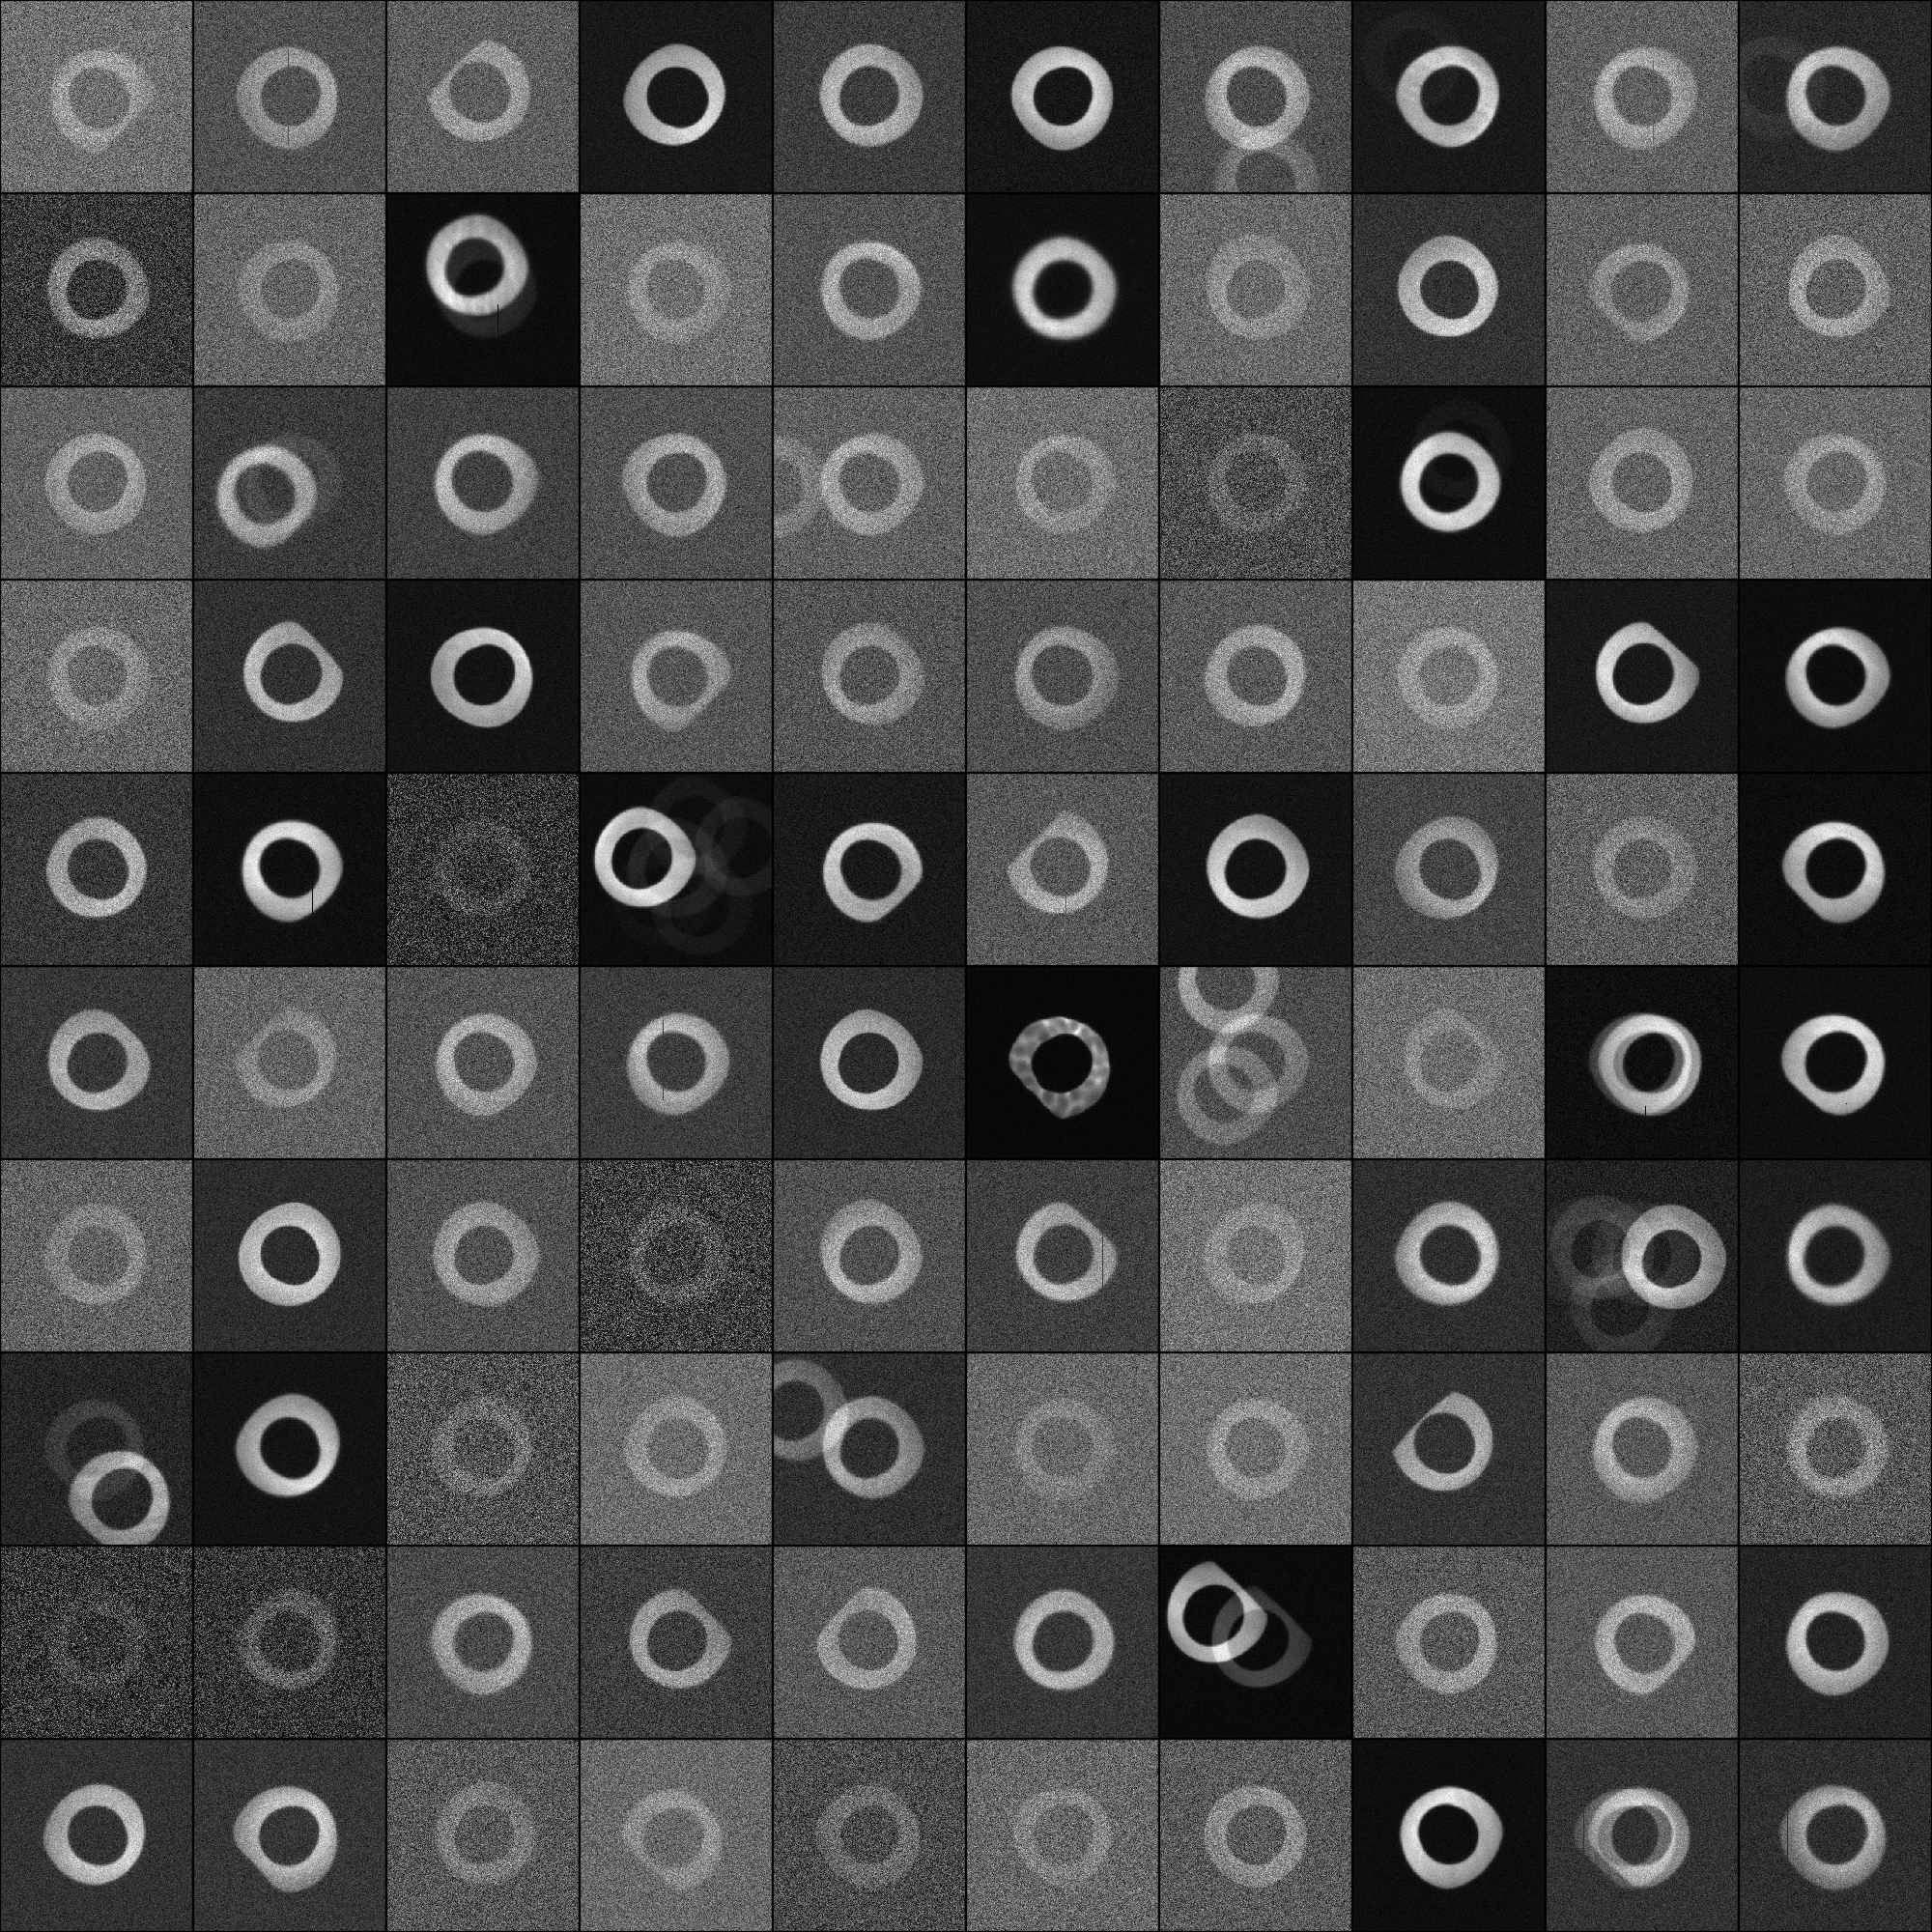
\includegraphics[width=\textwidth]{figs/simulating_donuts/huge_donut_box.png}
\end{tabular}
\end{center}
\caption[Example Donuts from Donut Dataset]{Example donuts from the training set. The different degrees of vignetting, missing columns, blending, and turbulence can be seen with the naked eye.\label{fig:donutbox}}
\end{figure}

\section{Full Visit Dataset}

The full problem involves going from $n$ donut images and positions to the 54 coefficients $\beta$,

\begin{equation}\label{eqn:blackbody}
(D_1,r_1), \dots, (D_n, r_n) \to \alpha_1, \dots, \alpha_n \to \beta
\end{equation}

\noindent In addition to the donut dataset, we also need a dataset of full visits, where each visit contains many donut images, so that we can assess how well our framework predicts $\beta$.

Each sample in this dataset consists of all the donut images and positions in the observation, plus the full optics wavefront $\beta$. We used the last 497 observations from the scheduler simulations for the observations. For each visit, we simulated all the stars, and blends, from the Gaia catalog that fall on the corner wavefront sensors. The mean, median, and maximum number of sources in a sample is 787, 222, and 4,998 respectively. Figure \ref{fig:sensordonut} shows an example sample.

\begin{figure} [!htbp]
\begin{center}
\begin{tabular}{c}
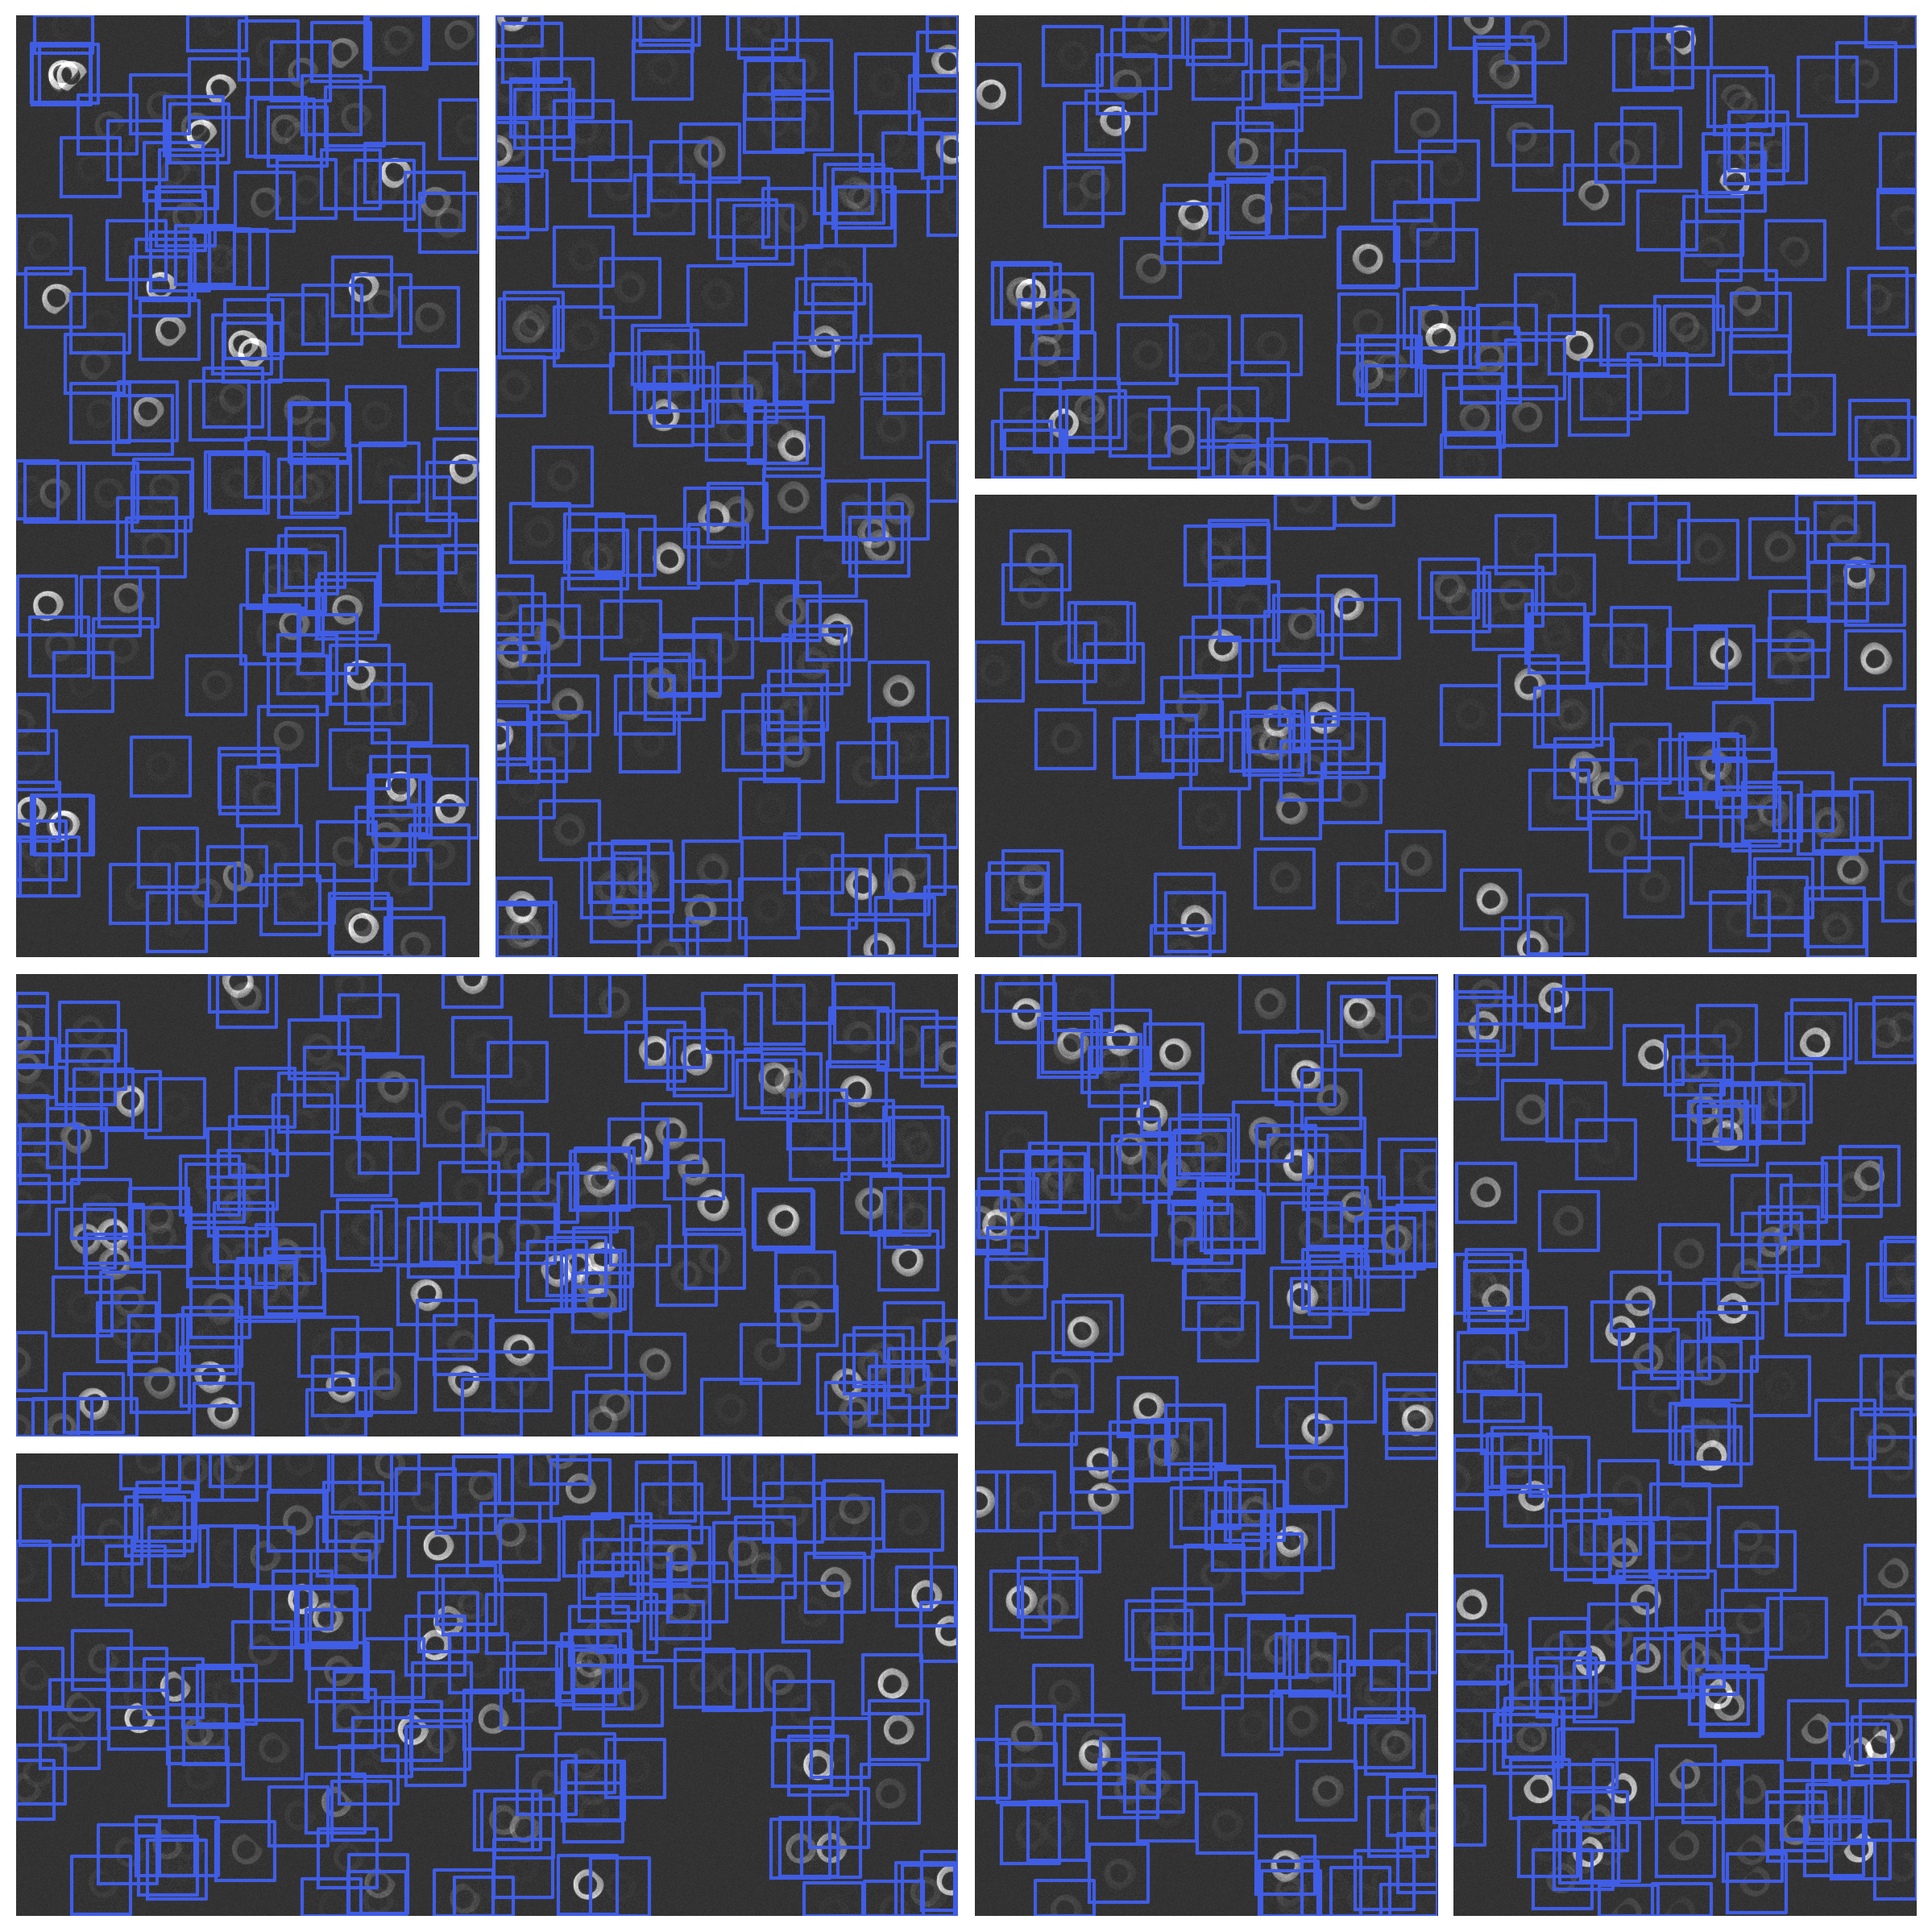
\includegraphics[width=\textwidth]{figs/simulating_donuts/sensors_and_donuts.png}
\end{tabular}
\end{center}
\caption[Example Full Visit Sample]{The eight wavefront sensor half-chips in an example sample from the full visit dataset. This sample contains 1112 donut images which are highlighted in blue boxes. \label{fig:sensordonut}}
\end{figure}

All the donuts within a single observation are simulated with the same atmosphere and sky background. Otherwise, each star in the observation is simulated in the same manner as the donuts dataset described above. For each observation, we used the batoid framework to compute the optics wavefront double Zernike coefficients for the perturbed telescope instance.

The largest difference between observations is the density of sources in the field. The number of sources in a sample ranges from 111 to 4998. On average, 32 percent of the sources are blends. However, for the crowded fields this number can be over 90 percent. Figure \ref{fig:blendfraction} shows how the fraction of sources that are blends increases with the total number of sources in the visit. Thus, while for less crowded fields ample un-blended stars are available, for crowded fields, the wavefront sensing algorithm's ability to process blends is critical.

\begin{figure} [!htbp]
\begin{center}
\begin{tabular}{c}
\includegraphics[width=\textwidth]{figs/simulating_donuts/blendfraction.png}
\end{tabular}
\end{center}
\caption[Fraction of Blended Sources]{The fraction of sources that are blends versus the total number of sources for the 497 visits in the full visit dataset.\label{fig:blendfraction}}
\end{figure}

% Full title as you would like it to appear on the page
\chapter{Training a Convolutional Neural Network To Predict The Local Wavefront}
\label{chap:cnn}
\chaptermark{Training a CNN}

\section{Network Architecture}

[latest network architecture]
* table with components

\section{Training, Validation, and Testing}

[training curve]
[performance distribution]
[donut panel]
*table

\section{Advanced Insights}

[attention]
[recover zernikes]
[adversarial]

% Full title as you would like it to appear on the page
\chapter{Interpolating The Global Wavefront with Least Squares}
\label{chap:interp}
\chaptermark{Interpolating The Global Wavefront}

\epigraph{In questions of science, the authority of a thousand is not worth the humble reasoning of a single individual.}{Galileo Galilei}
% \epigraph{The first principle is that you must not fool yourself and you are the easiest person to fool.}{Richard P. Feynman}

\section{The Interpolation Geometry}

In the second step, we interpolate the global wavefront from the local wavefront predictions from the first step. We interpolate the global wavefront coefficients $\beta_{jk}$ based on the predictions $\alpha$ from the previous step. More explicitly, we use ordinary least squares (LS) to solve

\begin{equation*}
\text{LS}(\alpha(x_1,y_1), \dots, \alpha(x_n,y_n)) \to \beta_{jk} \text{ such that } W(u,v,x,y) = \sum_{j=4}^{21}\sum_{k=1}^3\beta_{jk}Z_j(u,v)Z_k(x,y)
\end{equation*}

In the previous step, the 18 predictions $\{\alpha_4(x_i, y_i), \dots, \alpha_{21}(x_i,y_i)\}$ for a source image $D$ at position $(x_i,y_i)$. In this step, we start by aggregating the predictions for a single coefficient $j$ for all $n$ donuts in the field of view of the observation, or $\{\alpha_j(x_1, y_1), \dots, \alpha_{j}(x_n,y_n)\}$. Then the problem reduces to minimizing the distance between the $\alpha_j$ estimates and $\sum_{k=1}^3\beta_{jk}Z_k(x,y)$ for each index separately. Figure \ref{fig:rafts} shows the true and predicted $\alpha_4$ values on the four wavefront sensors. 

\begin{figure}[!htbp]
\begin{center}
\begin{tabular}{c}
\includegraphics[width=\textwidth]{figs/interp/rafts.png}
\end{tabular}
\end{center}
\caption[Local Wavefront Predictions Across Four Wavefront Sensors]{The two rows correspond to the true ($\alpha_4^{\text{true}}$) and predicted ($\alpha_4^{\text{predicted}}$) $Z_4$ coefficients. The four columns correspond to the four corner wavefront sensors. The colormap is in units of waves.\label{fig:rafts}}
\end{figure}

The first three Zernike coefficients establish a plane. Thus we are effectively fitting a plane by the three coefficients along the $k$ index, for each local wavefront Zernike coefficient, or $j$ index. Figure \ref{fig:fieldols} shows how $\beta_{41}, \beta_{42}, \beta_{43}$ are fit from the local $\alpha_4$ predictions.

\begin{figure}[!htbp]
\begin{center}
\begin{tabular}{c}
\includegraphics[width=\textwidth]{figs/interp/fieldols.png}
\end{tabular}
\end{center}
\caption[Fitting Global $\beta_{41}, \beta_{42}, \beta_{43}$ From Local $\alpha_4$ Predictions]{\textit{Left:} the predicted coefficients $\alpha_4^{\text{pred}}$ from Figure \ref{fig:rafts} shown at their corresponding field locations within the field of view. \textit{Right:} the plane characterized by the three fit double Zernike coefficients $\beta^{\text{pred}}_{41},\beta^{\text{pred}}_{42}, \beta^{\text{pred}}_{43}$. The two circles represent the field of view of the Rubin Observatory. \label{fig:ls-intuition}}
\end{figure}

The explicit minimization is 

\begin{equation*}
\label{eq:objective}
\text{min}_{\beta}\left|\left| \begin{bmatrix}\alpha_j(x_1,y_1) \\ \vdots \\ \alpha_j(x_n,y_n) \end{bmatrix} - \begin{bmatrix}Z_1(x_1,y_1) & Z_2(x_1,y_1) & Z_3(x_1,y_1) \\ \vdots & \vdots & \vdots\\  Z_1(x_n,y_n) & Z_2(x_n,y_n) & Z_3(x_n,y_n)\end{bmatrix} \begin{bmatrix}\beta_{j1} \\ \beta_{j2} \\ \beta_{j3} \end{bmatrix}\right|\right|_2
\end{equation*}

\noindent which we solve with ordinary least squares. Letting $\alpha_j, Z, \beta_j$ be the vectors and matrices from the equation above, we have the analytic solution $\beta_j = (Z^TZ)^{-1}Z^T\alpha_j$. After solving this equation for each $j$, we have $\beta_{jk}$ for $4 \leq j \leq 21$ and $1 \leq k \leq 3$. In the next section we describe a few variations to this basic framework.

\section{Evaluating Different Interpolation Strategies}

The interpolation is comprised of three steps that are reminiscent of a standard data query: select, reduce, and fit. The \textit{select} step decides which donuts and corresponding local estimates to use in the interpolation. The \textit{reduce} step, which is typically skipped, reduces these estimates across a wavefront sensor. The \textit{fit} step fits the local coefficients to a global Zernike basis based on the provided loss function.

We examine multiple variations in each of these steps to find which combination works best. We explore selecting donuts from all the sources (stars and blends), from only the non-blended stars (stars), the non-blended 10 brightest stars per chip (brightest stars), and using the true labels (labels). The results on the true labels provide a sanity check and bound the performance we can expect to achieve with alternatives. 

We also analyze two variations in the reduce step. Either we make no changes to estimates and effectively skip this step, or we take the median of the estimates on each chip. In the median case, we would then fit against the four points corresponding to the four sensors in the fit step. 

We explore three different fitting strategies. The $\ell_1$, or absolute loss, is convex and can be found with an iterative optimization algorithm. The $\ell_2$, or least squares loss, has an analytic solution. This has the added benefit of making error propagation analytic as well. Finally, the Huber loss $\ell_h$ is similar to the $\ell_2$ for samples with small error but scales like $\ell_1$ for large error. Thus it is similar to $\ell_2$ but less sensitive to outliers.

The results of these variations, applied to the local wavefront estimates from the neural network, applied to the full visit dataset, are shown in Table \ref{tab:variations}. We compare the true global wavefront and the residual global wavefront, where the residual is the true wavefront minus the interpolated optics wavefront. The residual wavefront is smaller than the original wavefront for all the samples in the majority of select-reduce-fit variations. The consistency of the improvements makes our method an attractive candidate for deployment.

\begin{table}
{
\begin{center}
\begin{tabular}{|c|c|c|c|r|}
\hline
 & Median &  & \multicolumn{1}{|c|}{\% Samples} & \multicolumn{1}{|c|}{Relative}  \\
Select & Reduce & Fit & \multicolumn{1}{|c|}{Improved} & \multicolumn{1}{|c|}{Residual} \\
\hline
 &  & $\ell_1$ & $ 99.6$ & $ 0.48 \pm  0.13$\\
Stars & & $\ell_2$ &  $ 99.8$ & $ 0.49 \pm  0.12$\\
and&  & $\ell_{\text{h}}$ &  $ 100.0$ & $ 0.48 \pm  0.12$\\
Blends& \checkmark & $\ell_{1}$ &  $ 97.8$ & $ 0.67 \pm  0.14$\\
& \checkmark & $\ell_{2}$ &  $ 100.0$ & $ 0.46 \pm  0.12$\\ 
\hline
&   & $\ell_1$ &  $ 99.8$ & $ 0.44 \pm  0.11$\\ 
&   & $\ell_2$ &  $ 100.0$ & $ 0.43 \pm  0.10$\\ 
Stars&  & $\ell_{\text{h}}$ &  $ 100.0$ & $ 0.43 \pm  0.10$\\
& \checkmark  & $\ell_{1}$ &  $ 97.2$ & $ 0.64 \pm  0.14$\\
& \checkmark  & $\ell_{2}$ &  $ 99.8$ & $ 0.41 \pm  0.11$\\
\hline
& & $\ell_1$ &  $ 99.6$ & $ 0.37 \pm  0.13$\\ 
Brightest& & \textcolor{blue}{$\ell_2$} & \textcolor{blue}{$ 100.0$} & \textcolor{blue}{$ 0.34 \pm  0.12$}\\ 
Stars& & $\ell_{\text{h}}$ &  $100.0$ & $ 0.34 \pm  0.12$\\ 
& \checkmark & $\ell_{1}$ &  $97.2$ & $ 0.60 \pm  0.16$\\ 
& \checkmark & $\ell_{2}$ &  $100.0$ & $ 0.35 \pm  0.12$\\
\hline
& & $\ell_1$ &  $ 100.0$ & $ 0.13 \pm  0.05$\\ 
Labels & & \textcolor{red}{$\ell_2$} & \textcolor{red}{$ 100.0$} & \textcolor{red}{$ 0.06 \pm  0.02$}\\
& & $\ell_{\text{h}}$ &  $ 100.0$ & $ 0.08 \pm  0.04$\\ 
\hline
\end{tabular}
\end{center}
}
\caption[Select-Reduce-Fit Results]{Each row contains the results for a different combination of select, reduce, and fit steps. The penultimate column contains the percentage of the number of samples where the residual improved. The final column contains the relative residual: the total magnitude of the residual divided by the total magnitude of the true wavefront. The best variation on neural network estimates is highlighted in \textcolor{blue}{blue}. The best variation on the true label estimates is highlighted in \textcolor{red}{red}.}
\label{tab:variations}
\end{table}

This experiment also taught us that more data is not always better. Ignoring the blended donuts leads to a clear improvement in performance. So does ignoring all but the brightest stars. This suggests that we should prioritize making accurate predictions on the best donuts, perhaps at the expense of making consistent estimates on all the donuts. It also may have consequences for wavefront sensing in crowded fields where almost all of the donuts are blended.

We can also draw conclusions about the variations. Taking the median and fitting with the $\ell_1$ norm appears to discard too much information. We also see that the benefit of using median with the $\ell_2$ norm goes away as the select becomes more selective. This is likely because the outliers, which the median reduce suppresses, get filtered and are no longer an issue. The $\ell_{h}$ norm also seems to do comparatively well on stars and blends, but loses this advantage on the more selective brightest stars selection. We conclude using the $\ell_2$ norm, with no median reduce, to fit the brightest stars, is the best variation.

We used this variation to explore how our framework performs in five scenarios. We used the relative residual $|\beta^{\text{res}}| / |\beta^{\text{true}}| = \sum_{jk}|\beta^{\text{true}}_{jk} - \beta^{\text{pred}}_{jk}| / \sum_{jk}|\beta^{\text{true}}_{jk}|$ to measure our algorithm's capability to reproduce the true global wavefront. A value close to zero means the predictions match the true global wavefront almost perfectly; a value close to one means the predictions capture almost none of the true global wavefront. Figure \ref{fig:beta-results} shows the results.

\begin{figure}[!htbp]
\begin{center}
\begin{tabular}{c}
\includegraphics[width=\textwidth]{figs/interp/dist_defense2.png}
\end{tabular}
\end{center}
\caption[Relative Residuals In Different Scenarios]{The distributions of relative residuals in four different scenarios. The distributions from performing the interpolation over the labels with and without noise are shown in black. The distributions from performing the interpolation over the local wavefront predictions from the neural network with and without noise are shown in blue. \label{fig:beta-results}}
\end{figure} 

In the first scenario, we evaluated the second step of our algorithm on the true local wavefront labels from the first step. The relative residual is 6\%, which validates that our simulations are consistent and there are no sources of catastrophic numerical error. In the second scenario, we added uncorrelated Gaussian noise to each local wavefront coefficient. The variance of the noise for each coefficient was equal to the variance of the neural network error on that coefficient in the test data. Despite this noise, the relative residual remained very low at 10\%. This shows that our approach is not overly sensitive to uncorrelated noise.

In the third scenario, we fed the local wavefront predictions from the neural network to the second step. These have significant correlated error due to the atmosphere. The relative residual is 34\%, extremely promising, with a tight 12\% standard deviation. Furthermore, the right tail decays rapidly. Not a single relative residual is greater than one. Our framework improves the global wavefront on every observation in the full visit dataset!

In the fourth scenario we add noise as in the second scenario, effectively doubling the error. The relative residual increases slightly to 38\%. This suggests that the network is fairly robust to uncorrelated noise.

\section{Combined Runtime}

The run-time is another key advantage of our approach. It takes just under 4 seconds to process 811 donut images on a 2.4 GHz Intel Xeon CPU with a single Nvidia V100 GPU. It takes an additional 5 milliseconds to run the least squares optimization. The total processing time per donut image is 5 milliseconds; the total processing time per donut of the Rubin Observatory AOS under development is around 10 seconds\cite{2015Xin,2014Overiew}. Our scheme can process donuts 2,000 times faster, and is capable of processing 7,800 donuts in a single 39 second Rubin visit. The low latency allows it to process all the donuts in most observations.

\section{Image Quality Results}

The next step is to take this model and measure the repercussions of subtracting its estimate from the true wavefront on both the PSF FWHM and Strehl ratio \cite{strehl1895aplanatische}. We compute these by calculating the local wavefronts at the center and one corner of the focal plane. Then we take the fourier transform of the resulting pupil plane aberration to get the point spread function. The results for the original and corrected wavefronts are shown in Table \ref{tab:corrections}. 

\begin{table}
{
    \begin{center}
    \begin{tabular}{|l|l|c|c|}
    \hline
    State & Position & FWHM & Strehl\\
    \hline
    Before & Center & $0.288 \pm 0.034$ & $0.093 \pm 0.39$ \\
    After & Center & $0.211 \pm 0.005$ &  $0.555 \pm 0.207$\\
    \hline
    Before & Corner & $0.314 \pm 0.045$ & $0.074 \pm 0.32$\\
    After & Corner & $0.215 \pm 0.009$ & $0.400 \pm 0.184$\\
    \hline
    \end{tabular}
    \end{center}
}
\caption[Improvements To The Optics PSF FWHM And Strehl Ratio]{We measure the optics PSF FWHM and Strehl ratio on the original optics wavefront from the observation (Before), and the residual wavefront resulting from subtracting our wavefront estimate from the original optics wavefront (After). The Center position is at the center of the Rubin focal plane; the Corner position is at the center of the $R00$ wavefront sensor in the corner of the focal plane.}
\label{tab:corrections}
\end{table}

The optics PSF FWHM decreases considerably, especially when compared to the standard deviation of the original. The Strehl ratio increases in an even more extreme manner. Figure \ref{fig:vision} provides an illustrative example of how the improvements to the optics PSF from our method can improve image quality. We apply the Rubin optics PSF, before and after subtracting the optics wavefront estimated by our framework, to six classic Hubble Telescope images in the absence of other significant PSF contributions.

\begin{figure}[!htbp]
\begin{center}
\begin{tabular}{c}
\includegraphics[width=\textwidth]{figs/interp/results.png}
\end{tabular}
\end{center}
\caption[Illustrative Hubble Telescope Images After Correction From Our Framework]{An illustration of the effect of wavefront correction using our techniques on image resolution.  We use actual Hubble Space Telescope images to show the effect.  The Before images are degraded by the wavefront aberrations we have simulated.  The After images show their reconstruction after wavefront estimation and correction using the technique we describe in this paper. On the bottom two rows, we show the effective PSF, both before and after wavefront correction. The images have an angular extent of 3 arcseconds and the PSFs are displayed on a $0.16 \times 0.16$ arcsecond grid. \label{fig:results}}
\end{figure}

For the Rubin Observatory however, the PSF is dominated by the atmosphere, which as indicated cannot be corrected. For the Rubin observatory the assumed PSF width is of order 0.71 arcseconds, of which 0.65 is contributed by the atmosphere. Therefore, the improvement in the Strehl and image quality is not as dramatic. Nevertheless, this improvement is still important for use on nights with unusually good atmospheric seeing and also for applications that are especially sensitive to the PSF width.

% Full title as you would like it to appear on the page
\chapter{Error Covariance Fitting and Optimal Telescope Control}
\label{chap:err}
\chaptermark{Error and Control}

\epigraph{By failing to prepare, you are preparing to fail.}{Benjamin Franklin}

In this chapter, we transition from developing our wavefront sensing framework to showing how it can be used to optimally control a telescope like the Rubin Observatory. The connecting bridge is the error covariance matrix of the estimated global wavefront coefficients. In Section \ref{sec:error}, we show how our framework allows this covariance to be easily computed. Then in Section \ref{sec:optcont}, we show how we can use this in control simulations and assess different control strategies.

\section{Error Covariance Fitting}
\label{sec:error}

The key breakthrough is that since the interpolation step of our algorithm has a closed form, the error covariance is a closed form function of the error covariance of our local wavefront predictions from the first step. In order to do this we first fix the positions of the 10 brightest stars on each of the four sensors. For indexing, let $(x_1,y_1)$ be the first position on the first corner sensors, $(x_{11},y_{11})$ be the first position on the second sensor, ... and $(x_{31},y_{31})$ be the first position on the fourth sensor. Then we define $\gamma$ as

\begin{equation*}
\gamma = \begin{bmatrix}
\alpha_4(x_1,y_1)\\
\dots\\
\alpha_4(x_{10}, y_{10})\\
\alpha_5(x_1,y_1)\\
\dots\\
\dots \\
\alpha_{21}(x_{10},y_{10})\\
\alpha_4(x_{11}, y_{11})\\
\dots \\
\dots \\
\alpha_4(x_{21}, y_{21})\\
\dots \\
\dots \\
\alpha_4(x_{31}, y_{31})\\
\dots \\
\dots \\
\alpha_{21}(x_{40},y_{40})\\
\end{bmatrix}
\end{equation*}

\noindent Thus $\gamma \in \mathbb{R}^{720}$, where 720 stems from 10 positions, 4 sensors, and 18 coefficients. We also make the empirically confirmed assumption that the individual local wavefront coefficient predictions are zero centered. Then the error covariance between $\gamma_1, \gamma_2$ measures the error covariance of the $\alpha_4$ predictions across donut locations on the first wavefront sensors; the error covariance between $\gamma_1, \gamma_{11}$ measures the error covariance between the $\alpha_4$ and $\alpha_5$ predictions at the same donut position; the error covariance between $\gamma_1, \gamma_{181}$ measures the error covariance of the $\alpha_4$ predictions between positions on two different corner wavefront sensors. Thus a lot of different forms of covariance are encoded in the covariance between elements of $\gamma$. The full error covariance on the local wavefront predictions is $\Sigma_{\gamma} = \text{Cov}(\gamma, \gamma)$.

We assume that the error $\gamma$ is a multi-dimensional gaussian random variable. Then the covariance from the maximum likelihood estimate is $\Sigma_{\gamma} = (X - E[X])(X-E[X])^T$ where $X \in \mathbb{R}^{497 \times 720}$ such that $X_i = \gamma^{(i)}$ the local wavefront errors from the ith observation. Figure \ref{fig:large-cov} shows the local estimate covariance matrix. 

\begin{figure}[!htbp]
\begin{center}
\begin{tabular}{c}
\includegraphics[width=\textwidth]{figs/control/obs_cov_written_thesis.png}
\end{tabular}
\end{center}
\caption[Error Covariance Of Local Wavefront Estimates]{The error covariance matrix $\Sigma_{\gamma}$ for the local wavefront error estimates in units of waves.\label{fig:large-cov}}
\end{figure}

Recall that if $y = Bx$, then $\text{Cov}(y,y) = B\text{Cov}(x,x)B^T$. In our case we can define an $A$, such that $\beta = (A^TA)^{-1}A^T\gamma$. This $A$ is 

\begin{equation*}
A = \begin{bmatrix}
I_{18} \otimes \begin{bmatrix}Z_1(x_1,y_1) & Z_2(x_1,y_1) & Z_3(x_1,y_1) \\ \vdots & \vdots & \vdots \\  Z_1(x_{10},y_{10}) & Z_2(x_{10},y_{10}) & Z_3(x_{10},y_{10}) \end{bmatrix}\\
I_{18} \otimes \begin{bmatrix}Z_1(x_{11},y_{11}) & Z_2(x_{11},y_{11}) & Z_3(x_{11},y_{11}) \\ \vdots & \vdots & \vdots \\  Z_1(x_{20},y_{20}) & Z_2(x_{20},y_{20}) & Z_3(x_{20},y_{20}) \end{bmatrix}\\
I_{18} \otimes \begin{bmatrix}Z_1(x_{21},y_{21}) & Z_2(x_{21},y_{21}) & Z_3(x_{21},y_{21}) \\ \vdots & \vdots & \vdots \\  Z_1(x_{30},y_{30}) & Z_2(x_{30},y_{30}) & Z_3(x_{30},y_{30}) \end{bmatrix}\\
I_{18} \otimes \begin{bmatrix}Z_1(x_{31},y_{31}) & Z_2(x_{31},y_{31}) & Z_3(x_{31},y_{31}) \\ \vdots & \vdots & \vdots \\  Z_1(x_{40},y_{40}) & Z_2(x_{40},y_{40}) & Z_3(x_{40},y_{40}) \end{bmatrix}
\end{bmatrix}
\end{equation*}

\noindent where $I_{18} \in \mathbb{R}^{18 \times 18}$ is the identity matrix, $\otimes$ is the kronecker product, and $Z_i(x_j,y_j)$ is the $jth$ circular Zernike polynomial being evaluated at focal plane position $x_j,y_j$. Then the error covariance matrix for $\beta$ is $\Sigma_{\beta} = (A^TA)^{-1}A^T\Sigma_{\gamma}A(A^TA)^{-1}$. It is shown in Figure \ref{fig:small-cov}.

\begin{figure}[!htbp]
\begin{center}
\begin{tabular}{c}
\includegraphics[width=\textwidth]{figs/control/beta_cov_written_thesis.png}
\end{tabular}
\end{center}
\caption[Error Covariance Of Global Wavefront Estimates]{The error covariance matrix $\Sigma_{\beta}$ for the global wavefront error estimates in units of waves.\label{fig:small-cov}}
\end{figure}

The global wavefront covariance $\Sigma_{\beta}$, which can be computed based on the empirically determined $\Sigma_{\gamma}$, is a key advantage to our wavefront sensing framework. We can use this statistical error model to characterize the performance of the system through time.

\section{Optimal Control}
\label{sec:optcont}

We developed a simulator in order to assess different control strategies. The simulator simulates the global wavefront coefficients over discrete time steps. There are three steps at each time step. First, a perturbation is applied. In practice, this would be caused by changes to the wind, gravitational stress, thermal gradients, etc. Second, the global wavefront prediction is made with the error covariance from the previous section. Third a control strategy is applied with this estimate. Figure \ref{fig:control-algo} summarizes the simulator algorithm. 

\begin{figure}[!htbp]
\begin{center}
\begin{tabular}{c}
\includegraphics[width=3in]{figs/control/algo.png}
\end{tabular}
\end{center}
\caption[Control Simulator Algorithm]{The control simulator algorithm. The sequence of perturbations, error covariance matrix, and control strategy are passed by the client.\label{fig:control-algo}}
\end{figure}

We used this simulator to test four different control strategies. The first is the null control strategy which does not make any changes to the control parameters, or 

\begin{equation*}
\text{Control-Null}(\hat{\beta}_i) = \hat{\beta}_i
\end{equation*}

\noindent This is useful for null tests.

The second is a gain controller. It makes the update 
\begin{equation*}
\text{Control-Gain}(\hat{\beta}_i) = g \cdot \hat{\beta}_i
\end{equation*} 
\noindent where $g$ is the gain, which is typically less than 1. When $g=1$, this reduces to the null controller.

The third is a proportional-integral-derivative (PID) controller. It extends the gain controller with two additional additive terms. One term accumulates the estimates, the other uses the difference between the current and previous estimates as a proxy for a derivative. It makes the update

\begin{equation*}
\text{Control-PID}(\hat{\beta}_i) = c_p \cdot \hat{\beta}_i + c_i \sum_{j=1}^i \hat{\beta}_j + c_d \cdot (\hat{\beta}_i - \hat{\beta}_{i+1})
\end{equation*}

\noindent where $c_p, c_i, c_d$ are the configurable model parameters. When $c_i = c_d = 0$ it reduces to the gain controller.

The fourth is a linear-quadratic-gaussian (LQG) controller. In control theory, the separation principle says that the problem of designing an optimal controller for a stochastic system can be decomposed into (i) an optimal estimator of the state and (ii) an optimal deterministic controller. LQG adheres to this decomposition. A Kalman filter (or linear-quadratic state estimator) is used for state estimation and a linear-quadratic regulator is used for control. For our discrete time problem, the update is

\begin{align*}
\text{Control-LQC}(\hat{\beta}_i) &= K_i \cdot x_i\\
x_{i+1} &= x_i - u_i + L_i (\hat{\beta}_i - x_i + u_i)\\
x_0 &= \hat{\beta}_0\\
L_i &= P_i(P_i + \Sigma_{\beta} + V)^{-1}\\
P_{i+1} &= P_{i} - P_i (P_i + \Sigma_{\beta} + V)^{-1} P_i + V\\
P_0 &= \Sigma_{\beta} + V\\
K &= (S_h + R)^{-1} S\\
S_{i+1} &= S_i - S_i (S + R)^{-1}S + Q\\
S_0 &= Q\\
\end{align*}

\noindent where $Q,R,V$ and the horizon $h$ are configurable parameters.

In order to make the sequence of perturbations in the simulator as realistic as possible we developed code to convert contiguous observations from OpSim into sequences of perturbations. We use two types of perturbations: Jump and Box. 

Jump perturbations are applied once at a specific time step. They are parameterized by a time step and scale. The 56-dimensional global wavefront perturbation is drawn from a zero-mean multivariate normal distribuation. The covariance is $\Sigma_{\beta}$ times the scale. 

Box perturbations are parameterized by a step, duration, and scale. It begins at the step time step and lasts for the duration number of time steps. At each time step, the 56-dimensional global wavefront perturbation is drawn from a zero-mean multivariate normal distribuation. The covariance is $\Sigma_{\beta}$ times the scale. It is worth noting that for each timestep within the duration, a different perturbation is drawn and applied. Table \ref{tab:conversion} shows how we convert OpSim sequences of observations into sequences of perturbations.

\begin{table}
{
\begin{center}
\begin{tabular}{|c|c|}
\hline
Observation & Perturbation\\
\hline
First 50 Observations & Box(start=0, duration=50, scale=2)\\
Last 50 Observations & Box(start=end-50, duration=50, scale=2)\\
Slew $> 5$ & Jump(step=step, scale=5)\\
Slew $> 20$ & Jump(step=step, scale=100)\\
Filter Change & Jump(step=step, scale=20)\\
\hline
\end{tabular}
\end{center}
}
\caption[Observation To Perturbation Conversions]{The mapping between catalog observations and their corresponding perturbations for the control simulator.}
\label{tab:conversion}
\end{table}

Each of the control strategies has parameters. We randomly selected 11 nights within the 10 year observing period for Rubin. We convert each of these nights into a sequence of perturbations for the control simulator. Then we fit the control strategy parameters on the first 10 nights, and evaluate them on the held out final night. The penalty combines the norm of the state, which is zero in the nominal state, and the size of the update.

\begin{equation*}
\text{Penalty} = ||\beta_{i+1}||_2^2 + \frac{1}{2}||\text{Control}(\hat{\beta}_i)||_2^2
\end{equation*}

For the gain controller, we found a gain of 0.39 was optimal. For the PID controller, we found $c_p = 0.37, c_i= 5.4\times 10^{-06}, c_d=.15$ was optimal. For the LQG controller, we found $Q = 0.84 \cdot I_{56}, R=0.88\cdot I_{56}$ with a fixed horizon $h=5$ and $V$ equal to the covariance of the state difference between steps with the null controller on the 10 training nights. The results on the final test night are shown in Figure \ref{fig:control-results}.

\begin{figure}[!htbp]
\begin{center}
\begin{tabular}{c}
\includegraphics[width=\textwidth]{figs/control/control_results.png}
\end{tabular}
\end{center}
\caption[Controller Results]{Left: the penalty of the different controllers through time on the test night. Right: the distributions of the penalties. \label{fig:control-results}}
\end{figure}

The first thing to note is that the performance of the three non-trivial controllers is very similar. The cumulative penalty for the different methods is 1901.78, 16.22, 15.61, and 16.92 for the null, gain, PID, and LQG controllers respectively. It seems like the PID controller best balances the positives from its sophistication and parameterization with the negatives that can arise from overfitting. 

As of yet, there has not been an investigation of the tradeoffs between different control strategis for Rubin. The current plan is to spend time during commissioning to take data and develop a strategy on the mountain. However, each extra day on the mountain not only delays the survey but also runs up the project budget. The framework we have presented here
has the potential to save this critical commissioning time by enabling this work on the mountain to be done now, with this framework. 

% Full title as you would like it to appear on the page
\chapter{Conclusions}
\label{chap:conclusion}
% Short title that appears in the header of pages within the chapter
\chaptermark{Conclusions}
\epigraph{Don't be afraid to give up the good to go for the great.}{John D. Rockefeller}

In this dissertation, we gave readers a comprehensive tour of our new two step wavefront sensing framework. 

In Chapter \ref{chap:new_paradigm}, we provided an overview of our framework. We started by describing the limitations of existing methods. Then we described the key conceptual breakthrough in our framework, that wavefront sensing can be decomposed into two sub-problems. The first sub-problem is to use a neural network to predict the local wavefront. The second sub-problem is to interpolate the global wavefront, represented by double Zernike polynomials, from the local wavefront estimates. We also demonstrated how 90\% of the aberration power is concentrated in the lowest three field Zernike polynomials, which makes the interpolation feasible. 

In Chapter \ref{chap:aos}, we covered the Rubin Observatory and its active optics system. We described the components of the telescope and the reduced 50 degrees of freedom that the active optics system strives to control.

Given that the Rubin Observatory is currently under construction, this work critically depends on high fidelity simulations. In Chapter \ref{chap:sim}, we described all the relevant physical effects and how they are modelled in our simulations. We also introduced the donut dataset and full visit dataset. We hope that these datasets can continue to serve as a research resource and benchmark for comparison moving forward. 

In Chapter \ref{chap:cnn}, we described how we trained a convolutional neural network to predict the local wavefront. After stepping through the architecture in detail, we explain the training process and assess the network's performance. We also characterized different potential sources of error. Ultimately our model made state of the art wavefront predictions. We believe this task, and our approach using a neural network to solve it, can serve a valuable component in many other wavefront sensing and optics algorithms.

In Chapter \ref{chap:interp}, we described how least squares is used to interpolate the global wavefront. We explored many select-reduce-fit combinations and found that using only the brightest stars, without reducing within a wavefront sensor, with an $l_2$ fit gave the best results. Our algorithm improved the wavefront in all 497 observations in the full visit dataset. It also reduced the total magnitude of the optics global wavefront by 66\%, the optics PSF FWHM by 27\%, and increased the Strehl ratio by a factor of 6. The illustrative Hubble images provide a sense of how much impact this image quality improvement can have on the downstream science applications. 

In Chapter \ref{chap:err}, we described our telescope control simulator. We evaluated the performance of three classic optimal control strategies with varying degrees of sophistication. This framework we have built on top of our wavefront sensing algorithm enables research on telescope control strategies to begin now, and potentially save time on the mountain during the commissioning of the Rubin Observatory. 

Finally, in addition to achieving incredible performance, it is worth stressing that our algorithm has many practical advantages.

\begin{itemize}
\item \textbf{Transparency:} 2 steps.
\item \textbf{Robustness:} 2x noise leads to 11\% performance degradation.
\item \textbf{Low Latency:} 5 milliseconds per donut.
\item \textbf{High Bandwidth:} 7,800 donuts in 39 seconds.
\end{itemize}

\noindent There is no existing alternative that achieves this combination of properties. Our two step wavefront sensing algorithm has the potential to improve image quality on multiple current and upcoming wide-field telescopes. We hope physicists continue to be receptive to interdisciplinary collaborations with those from applied mathematics and machine learning backgrounds. Leveraging these techniques has the potential to continue advancing many experiments and investigations in physics and cosmology. 
% \part{Star Trail Photometry}
% \part{Quantum Metric Learning}

% \include{ch_conclusion}

% uncomment below if you have an appendix
% \appendix
% \chapter{A Long Proof}

\bibliographystyle{unsrt}  % can change to fit your field e.g. pnas2009
\bibliography{mybib}  % no .bib extension necessary

% adds a non-numbered signature page at end (for printing on ACID-FREE paper)
% (remember to comment out when submitting final version)
\onlinesignature

\end{document}
